\documentclass[a4paper, 11pt, oneside]{report} 

\newcommand{\plogo}{\fbox{$\mathcal{PL}$}} 
\usepackage{graphicx}
\usepackage{graphics}
\usepackage{float}
\usepackage[table,xcdraw]{xcolor}
\usepackage[utf8]{inputenc} 
\usepackage[T1]{fontenc} 
\usepackage{fouriernc} 
\usepackage{subcaption}
\usepackage{tikz}
\usepackage{pgfplots}
\usepackage{graphics}
\usepackage{longtable}
\usepackage[nottoc]{tocbibind}
\usepackage{url}
\usepackage{hyperref}
\usepackage{amsmath}
\usepackage{lipsum}
\pgfplotsset{compat=1.18}
\usetikzlibrary{arrows.meta, positioning, shapes.geometric}

\begin{document} 	
	\begin{titlepage} 
		
		\centering 
		
		\vspace*{\baselineskip} 
		
		{\scshape\Large \textbf{Real-Time Yoga Pose Detection and Correction Platform}} \\
		\vspace{\baselineskip}
		{\large A report submitted for the course named Project I (CS3201)} \\
		
		\vspace*{4\baselineskip}
		
		Submitted By \\
		\vspace{0.5\baselineskip}
		{\scshape\Large Thota Siva Sankar Rao} \\
		{\large SEMESTER VI} \\
		{\large 220101074} \\
		
		\vspace{2\baselineskip}
		
		Supervised By \\
		\vspace{0.5\baselineskip}
		{\scshape\Large Dr. Rajkumari Bidyalakshmi Devi} \\
		
		\vspace{2\baselineskip}
		
		\vfill
		
		\begin{center}
			
\includegraphics[width=5cm]{report_file/iiit manipur.png}
		\end{center}
		
		{\scshape\Large Department of Computer Science and Engineering} \\
		{\scshape\Large Indian Institute of Information Technology Senapati, Manipur} \\
		{\large April, 2026}
	
\end{titlepage}

%----------------------------------------------------------------------------------------

\begin{center}
   { \LARGE \textbf{Declaration}}
\end{center}
\vspace{1cm}
In this submission, I have expressed my idea in my own words, and I have adequately cited and referenced any ideas or words that were taken from another source. I also declare that I adhere to all principles of academic honesty and integrity and that I have not misrepresented or falsified any ideas, data, facts, or sources in this submission. If any violation of the above is made, I understand that the institute may take disciplinary action. Such a violation may also engender disciplinary action from the sources which were not properly cited or permission not taken when needed.

\vspace{2cm}
\noindent Thota Siva Sankar Rao \\
220101074 \\
DATE: 25-04-2026

\newpage

\begin{center}
	\thispagestyle{empty}
		
		\begin{table}[H]
			\centering
			\begin{tabular}{l}
				Department of Computer Science and Engineering \\
				Indian Institute of Information Technology Senapati, Manipur \\
			\end{tabular}
		\end{table}
		\par\noindent\rule{\textwidth}{0.4pt}
		\vspace{0.5cm}
		\noindent \textbf{Dr. Rajkumari Bidyalakshmi Devi} \\
		Assistant Professor, CSE, IIIT Manipur \\
		Email: \href{mailto:rajkumari@iiitmanipur.ac.in}{rajkumari@iiitmanipur.ac.in} \\
		Contact No: +91 xxxxx xxxxx \\
		
		\vspace{2cm}
		{\huge \textbf{To Whom It May Concern}} \\
		\vspace{1cm}
		
		\large{This is to certify that the project report entitled \textbf{``Real-Time Yoga Pose Detection and Correction Platform,''} submitted to the department of Computer Science and Engineering, Indian Institute of Information Technology Senapati, Manipur in partial fulfilment for the award of degree of Bachelor of Technology in Computer Science and Engineering is a record of bonafide work carried out by \textbf{Thota Siva Sankar Rao} bearing roll number \textbf{220101074} for the course Project I (CS3201).}\\
		
		\vspace{2cm}
		\noindent Signature of the Supervisor \\
		\textbf{(Dr. Rajkumari Bidyalakshmi Devi)} \\
		
		\vspace{1.5cm}
		\noindent Signature of the Examiner 1 ............................ \\
		\noindent Signature of the Examiner 2 ............................ \\
		\noindent Signature of the Examiner 3 ............................ \\
		\noindent Signature of the Examiner 4 ............................ \\
	\end{center}
\newpage
 

\begin{abstract}
Yoga is a globally practised discipline that requires precise body alignment for maximum therapeutic benefit and injury prevention. Access to expert instructors remains limited, particularly for home practitioners. This project presents a real-time AI-powered Yoga Pose Detection and Correction Platform that acts as a fully automated virtual yoga trainer operable via a standard webcam.

The system integrates three core components: (1) a MobileNetV2-based convolutional neural network, trained using two-stage transfer learning on a five-class yoga pose dataset, achieving a test accuracy of \textbf{88.94\%}; (2) a Google MediaPipe Pose Landmarker that extracts 33 three-dimensional body landmarks in real time, with Exponential Moving Average (EMA) smoothing applied to eliminate detection jitter; and (3) a biomechanical pose rules engine that computes joint angles at eight key joints and compares them against an ideal angle database to produce per-joint correctness scores and actionable corrective messages.

A priority-based text-to-speech voice engine speaks the most critical correction at each interval. A five-state finite state machine automates a complete guided yoga routine, advancing through five poses (Downward Dog, Goddess, Plank, Tree, and Warrior II) only after the user achieves and holds a correctness score of at least 75\% for 10 seconds. The system operates entirely offline on commodity hardware at 15--20 frames per second, with no microphone or internet connection required.

Results demonstrate the feasibility of automated, real-time pose coaching using open-source frameworks, and the architecture is designed to be extensible to a broader pose vocabulary and mobile deployment.
\end{abstract}

\pagebreak
	

        \begin{center}
            { \LARGE \textbf{Acknowledgement}}
        \end{center}
	\vspace{2cm}
	I would like to express my sincere gratitude to \textbf{Dr. Rajkumari Bidyalakshmi Devi}, Project Coordinator, Department of Computer Science and Engineering, IIIT Manipur, for her constant guidance, encouragement, and valuable insights throughout the course of this project.

	I am grateful to the faculty of the Department of Computer Science and Engineering at the Indian Institute of Information Technology Senapati, Manipur, for providing the academic foundation and resources necessary to undertake this project.

	I would also like to acknowledge the open-source community behind TensorFlow, MediaPipe, and OpenCV, whose tools made this project possible.

	Finally, I thank my family and peers for their unwavering support and motivation.
	
	
	\vspace{1cm}
	
	\hspace{7cm}
	\tableofcontents
	\listoffigures
        \listoftables
	\chapter{Introduction}
	
\section{Introduction}
Yoga is a globally practiced discipline that requires precise body alignment for maximum therapeutic benefit and injury prevention. However, access to expert instructors remains limited, particularly for home practitioners practicing in remote areas. Performing yoga poses incorrectly not only reduces the therapeutic benefit but also risks musculoskeletal injury. As the volume of digital wellness technology grows, there is an increasing need for reliable, real-time AI document and action intelligence. 

This project builds the SmartYoga platform to fill that gap: a full-stack, AI-powered system that acts as a virtual yoga trainer operable via a standard webcam. The system detects foundational poses, extracts skeletal landmarks, and provides real-time, priority-ranked voice feedback to help practitioners improve their form independently and safely.

\section{Problem Statement}
\subsection{Rationale for Automated Yoga Coaching}
Effective access to professional yoga guidance matters for injury prevention and health optimization. A home practitioner needs more than just a static video; they require a system that can "see" them and provide the same level of corrective feedback as a human instructor. The democratization of this expertise through AI is critical for making safe yoga practice accessible to those who cannot attend expensive physical studios.

\subsection{Barriers to Effective Real-Time AI Coaching}
Despite the capabilities of modern computer vision, several practical barriers remain:
\begin{enumerate}
    \item \textbf{Classification vs. Correction Gap:} Most existing systems can identify a pose (classification) but cannot determine if the alignment is anatomically correct (correction).
    \item \textbf{Information Overload:} Simultaneous reporting of multiple joint errors often confuses the user.
    \item \textbf{Landmark Jitter:} High-frequency noise in raw skeletal landmark detection makes overlays unstable and angle data unreliable.
    \item \textbf{Engagement Flow:} A lack of automated state management means users must manually pause or advance their routines, disrupting the meditative flow of yoga.
    \item \textbf{Hardware Constraints:} High-fidelity pose estimation often requires expensive GPUs, making it inaccessible on standard laptops.
\end{enumerate}

\subsection{Research Gap}
While human pose estimation (OpenPose, MediaPipe) has been studied extensively, the integration of these features into a production-grade application that combines classification, biomechanical rules, priority feedback, and automated routine management on commodity hardware remains a significant engineering challenge. Most existing open-source solutions are research scripts rather than cohesive, user-ready platforms.

\section{Motivation and Project Objectives}
The primary motivation behind this project is to build a secure, attributable, and deployable AI yoga coach that operates entirely locally on a 512MB RAM budget if necessary. The objectives are:
\begin{enumerate}
    \item Build a MobileNetV2-based pose classifier reaching over 88\% test accuracy.
    \item Integrate MediaPipe landmark detection with O(1) memory complexity for edge deployment.
    \item Design a priority-ranked voice feedback engine to provide actionable, non-disruptive guidance.
    \item Implement an automated five-pose guided routine using a Finite State Machine (FSM).
    \item Apply Exponential Moving Average (EMA) smoothing to eliminate landmark jitter for a professional-grade HUD.
    \item Enforce privacy by ensuring 100\% offline operation on standard hardware.
\end{enumerate}

\section{Scope of the Project}
The SmartYoga platform handles real-time video capture, skeletal analysis, and voice-driven coaching for five foundational poses: Downward Dog, Goddess, Plank, Tree, and Warrior II. This project includes the full lifecycle from data curation and CNN two-stage training to system integration and performance evaluation. Advanced features like 3D path tracking and multi-person analysis are identified as future work.

        \chapter{Literature Survey}
        
This chapter surveys existing work in yoga pose recognition, human body landmark detection, and AI-driven fitness coaching systems that provide relevant technical context for this project.

\section{Human Pose Estimation}
\subsection{OpenPose: Bottom-Up Multi-Person Tracking}
Human pose estimation is the computer vision task of detecting and tracking key anatomical landmarks (joints) from image or video data. Cao et al.~\cite{cao2017realtime} introduced OpenPose, a pioneering bottom-up approach that simultaneously detects body, hand, and face keypoints for multiple people in real time. The methodology utilizes Part Affinity Fields (PAFs) to learn the association between body parts, which allows the system to scale efficiently with the number of people in the frame. This established the precedent for skeleton-based body analysis in downstream classification tasks. However, OpenPose often requires significant GPU resources for optimal performance, making it challenging for deployment on standard consumer laptops without high-end hardware.

\subsection{MediaPipe BlazePose: High-Fidelity Tracking on Edge Devices}
Google's MediaPipe Pose~\cite{mediapipe2020} extended the capabilities of human pose estimation to edge and mobile devices. It utilizes a highly efficient BlazePose model that predicts 33 high-fidelity 3D body landmarks at real-time speeds. Unlike bottom-up approaches, BlazePose uses a top-down strategy starting with a person detector. The model is particularly optimized for single-person tracking with high temporal consistency, which is critical for fitness applications where the user is moving. This framework serves as the foundation of the landmark extraction module of this project due to its low latency and high accuracy on commodity CPUs.

\section{Deep Learning for Action and Pose Classification}
\subsection{MobileNet Architectures for Efficiency}
Convolutional Neural Networks (CNNs) have demonstrated exceptional performance in image classification tasks. However, large architectures like VGG16 or ResNet are often too computationally expensive for real-time mobile use. Howard et al.~\cite{howard2017mobilenets} addressed this by introducing MobileNets, a family of efficient CNNs designed for mobile and embedded vision applications. The core innovation is the use of depthwise separable convolutions, which significantly reduce the number of parameters and floating-point operations while maintaining competitive accuracy.

\subsection{MobileNetV2: Residual Blocks and Linear Bottlenecks}
Sandler et al.~\cite{sandler2018mobilenetv2} further improved this with MobileNetV2, incorporating linear bottleneck layers and inverted residual blocks. These architectural changes allow the network to preserve information across layers more effectively, significantly reducing parameter count while improving performance on benchmark datasets like ImageNet. These properties make MobileNetV2 ideal for real-time yoga classification on standard consumer hardware, where power and compute are limited.

\subsection{Transfer Learning and Domain Adaptation}
Transfer learning is the practice of taking a model pre-trained on a massive dataset, such as ImageNet~\cite{deng2009imagenet}, and fine-tuning it on a domain-specific task with a relatively smaller dataset. As systematically studied by Yosinski et al.~\cite{yosinski2014transferable}, features learned in the early layers of a CNN are often general (like edges and textures) and can be transferred across domains. By freezing these early layers and training only the top layers, and subsequently fine-tuning with a low learning rate, a model can achieve high accuracy on specialized tasks like yoga pose detection even with limited training data. This strategy is central to the training pipeline of this project.

\section{Yoga and Fitness AI Systems}
Several prior systems have addressed automated yoga or fitness pose analysis, providing a foundation for our research.

\subsection{The Yoga-82 Dataset}
Verma et al.~\cite{verma2020yoga82} introduced Yoga-82, a large-scale dataset for fine-grained yoga pose classification. This dataset includes 82 categories of yoga poses, organized in a hierarchical structure. While their work demonstrated the efficacy of deep feature extraction for semantic pose understanding, the focus was purely on static image classification. Their system does not provide real-time skeletal tracking or any form of corrective feedback, which limits its utility as a training assistant.

\subsection{AI Fitness Coaching Systems}
Academic and open-source projects have explored building AI fitness coaches using lighter-weight models like PoseNet. These systems are typically used for rep counting or simple form analysis in exercises like squats or pushups. While they succeed in flagging major deviations from ideal joint angles, they often lack a continuous, voice-guided training loop and sophisticated state management. This makes them more suitable for short-term feedback rather than a full, guided yoga session.

\subsection{Specialized Hardware Solutions}
Commercial products like StretchSense or YogAlign AI utilize IMU (Inertial Measurement Unit) sensors or specialized marker-based tracking to score poses. These systems offer high accuracy but require expensive, specialized hardware that is often cumbersome for the user to wear. Our project aims to achieve similar results using only markerless tracking from a standard webcam, making the technology accessible to a much broader audience.

\section{Structured Review of Key Prior Work}
Table~\ref{tab:litreview} provides a structured summary of the most relevant methods and datasets that informed the design of this project.

\begin{table}[H]
    \centering
    \caption{Structured review of key prior work: method, contribution, and project response}
    \begin{tabular}{|p{0.15\textwidth}|p{0.25\textwidth}|p{0.25\textwidth}|p{0.25\textwidth}|}
        \hline
        \textbf{Work} & \textbf{Method} & \textbf{Contribution} & \textbf{Project Response} \\
        \hline
        Cao et al. (OpenPose) \cite{cao2017realtime} & Bottom-up multi-person keypoint detection & Real-time multi-person skeletal tracking via PAFs & High GPU requirements; project uses MediaPipe for CPU-only edge performance. \\
        \hline
        MediaPipe (2020) \cite{mediapipe2020} & Top-down BlazePose landmarker & High-fidelity 33 landmark tracking on mobile/CPU & Adopted as the core foundation for landmark extraction and HUD logic. \\
        \hline
        Sandler et al. (MobileNetV2) \cite{sandler2018mobilenetv2} & Inverted residual blocks and linear bottlenecks & Efficient CNN architecture for mobile/embedded vision & Chosen as the classification backbone for real-time inference on laptops. \\
        \hline
        Verma et al. (Yoga-82) \cite{verma2020yoga82} & Hierarchical fine-grained classification & Large-scale dataset for yoga pose recognition & Purely classification-based; project adds biomechanical rules for correction. \\
        \hline
    \end{tabular}
    \label{tab:litreview}
\end{table}

\section{Summary of Identified Gaps}
The literature review identifies several critical gaps in existing AI yoga systems:
\begin{itemize}
    \item \textbf{Classification vs.\ Correction Gap:} Most datasets and models focus on identifying the pose name but fail to assess the quality of the practitioner's form.
    \item \textbf{Feedback Overload:} Existing corrective systems often report all form errors simultaneously, which can be overwhelming for a practitioner during a session.
    \item \textbf{Stability and Jitter:} Markerless tracking systems frequently suffer from high-frequency coordinate jitter, making real-time overlays visually distracting and unreliable for angle computation.
    \item \textbf{Instructional Flow:} There is a lack of cohesive, hands-free systems that guide a user through a multi-pose routine automatically without manual intervention.
\end{itemize}
This project addresses these gaps through the integration of a rules engine for form correction, a priority-based voice feedback mechanism, EMA coordinate smoothing, and a finite state machine for automated routine management.

        \chapter{Requirement Engineering}
        \section{Functional Requirements}
The functional requirements define the core behaviors and tasks the system must execute to fulfil its purpose as a virtual yoga trainer.

Firstly, the system is required to capture live video frames from a standard USB or built-in webcam. To ensure sufficient detail for landmark detection, the capture resolution is set to 1280$\times$720 pixels (720p). The application must handle individual frames in real time with minimal latency.

Secondly, the system must classify the yoga pose being performed from five target categories: Downward Dog, Goddess, Plank, Tree, and Warrior II. This classification must be reliable, with a confidence threshold set at $\geq 60\%$. Only when the classifier is confident in the pose identification should the subsequent correction logic be fully engaged for that specific pose.

Thirdly, the application must detect and track 33 body landmarks per frame using the MediaPipe Pose Landmarker. The system utilizes the "Lite" variant of the model via the MediaPipe Tasks API to balance accuracy and inference speed on CPU-based hardware.

Fourthly, the system computes eight key joint angles from the detected pixel-space landmarks. These joints include the left and right shoulders, elbows, hips, and knees. The computation must be robust to changes in the practitioner's distance from the camera.

Fifthly, the computed angles are compared against a predefined ideal-angle database. To account for natural variations in body types and flexibility, a tolerance of $\pm 15$ degrees is applied to the ideal ranges. If a joint falls within this range, it is considered correct.

Sixthly, the system produces a real-time correctness score (0\% to 100\%) based on the proportion of joints that are within the ideal range for the target pose. This score serves as a quantitative measure of the practitioner's form.

Seventhly, the application must speak the highest-priority corrective instruction via the offline TTS engine. To avoid overwhelming the user, instructions are spoken at intervals of at least 4 seconds, focusing on the joint with the largest deviation first.

Eighthly, the system guides the user through all five poses sequentially using a five-state training loop. This automated progression ensures that the user completes a full yoga routine without manual intervention.

Ninthly, the state machine advances to the next pose only after the user maintains a correctness score of $\geq 75\%$ for 10 continuous seconds. This "hold" requirement ensures that the practitioner has truly mastered the pose alignment.

Finally, the application must display all corrective instructions simultaneously in the on-screen footer HUD. This provides a visual fallback for the user and allows them to see the full list of required adjustments.

\section{Non-Functional Requirements}
Non-functional requirements specify the quality attributes and constraints of the system.

Performance is a critical constraint; the application must process and render at a minimum of 15 frames per second on a mid-range laptop CPU. High latency in the video feed or skeletal overlay would make the system unusable for real-time guidance.

Usability is addressed by ensuring the system requires no keyboard or mouse interaction once the session has started. The entire session is voice-driven and automated, allowing the practitioner to focus entirely on their yoga practice.

Reliability is ensured by the system's ability to maintain a stable state even when the user momentarily moves outside the camera frame. The skeletal and angle computation modules retain the last valid landmark state to prevent erratic feedback during brief occultations.

Portability is a key requirement, as the application must run on standard Windows or Linux machines with Python 3.10+ and a webcam. It is designed to be accessible without the need for specialized depth cameras or high-end GPUs.

Finally, the system must support offline operation. All core modules, including CNN inference, MediaPipe landmark detection, and the TTS engine, must function without an active internet connection to ensure user privacy and consistent performance regardless of network availability.

\section{Project Scope and Constraints}
The scope of this project is limited to the detection and correction of five foundational yoga poses. While the architecture is designed to be extensible, the current implementation focuses on providing a high-quality experience for these specific poses. The system is designed for single-person use in a home environment and assumes a relatively clear field of view for the webcam.

Constraints include the use of commodity hardware without dedicated GPUs for inference. This necessitates the use of efficient models like MobileNetV2 and MediaPipe Lite. Additionally, the system relies on the accuracy of the underlying pose estimator; if landmarks are poorly detected due to lighting or background clutter, the accuracy of the corrective feedback will be affected.

\section{Feasibility Study}
A feasibility study is conducted prior to implementation to ensure the proposed system is viable across technical, operational, and economic dimensions.

\subsection{Technical Feasibility}
Technical feasibility is assessed based on the ability of current hardware and software platforms to support high-speed inference and real-time visualization.

\begin{table}[H]
    \centering
    \caption{Technical Feasibility Overview}
    \begin{tabular}{|p{0.3\textwidth}|p{0.6\textwidth}|}
        \hline
        \textbf{Aspect} & \textbf{Details} \\
        \hline
        Tech Stack & Python 3.10+, TensorFlow/Keras, MediaPipe, OpenCV (all open-source). \\
        \hline
        Modular Design & Core logic (classification, landmark detection, HUD, logic) is decoupled into independent modules. \\
        \hline
        Edge Inference & Successfully tested on standard laptops; no external GPU or cloud dependence. \\
        \hline
        Landmark Precision & MediaPipe Tasks API delivers consistent tracking at 15--20 FPS on CPU. \\
        \hline
    \end{tabular}
    \label{tab:techfeas}
\end{table}

\subsection{Operational Feasibility}
The system is operationally feasible as it satisfies the requirements of a voice-driven, autonomous training assistant usable by practitioners of all technical levels.

\begin{table}[H]
    \centering
    \caption{Operational Feasibility Overview}
    \begin{tabular}{|p{0.3\textwidth}|p{0.6\textwidth}|}
        \hline
        \textbf{Aspect} & \textbf{Details} \\
        \hline
        User Interface & Minimalist HUD with visual indicators; requires no manual keyboard interaction. \\
        \hline
        Learning Curve & Intuitive guided routine with reference images and spoken feedback. \\
        \hline
        Deployment & Single-command execution (\texttt{python app.py}) for easy environment setup. \\
        \hline
    \end{tabular}
    \label{tab:opfeas}
\end{table}

\subsection{Economic Feasibility}
The system is economically efficient as it builds upon open-source frameworks and common hardware, eliminating specialized infrastructure costs.

\begin{table}[H]
    \centering
    \caption{Economic Feasibility Analysis}
    \begin{tabular}{|p{0.3\textwidth}|p{0.6\textwidth}|}
        \hline
        \textbf{Aspect} & \textbf{Details} \\
        \hline
        Software Cost & Zero (all dependencies are MIT/Apache/BSD-licensed). \\
        \hline
        Hardware Cost & Low (standard laptop with built-in webcam). \\
        \hline
        Maintenance & Minimal operational overhead; runs locally without subscription fees. \\
        \hline
    \end{tabular}
    \label{tab:econfeas}
\end{table}

\section{Software Requirement Specification (SRS)}
\subsection{Functional Requirements}
The functional requirements define the essential behaviors and tasks the SmartYoga platform must execute.

\begin{table}[H]
    \centering
    \caption{Functional Requirements Specification}
    \begin{tabular}{|c|p{0.25\textwidth}|p{0.55\textwidth}|}
        \hline
        \textbf{ID} & \textbf{Requirement} & \textbf{Description} \\
        \hline
        FR1 & Frame Capture & Capture 720p video from webcam at 15+ FPS. \\
        \hline
        FR2 & Pose Classification & Identify one of 5 target poses using CNN (threshold $\geq 60\%$). \\
        \hline
        FR3 & Landmark Tracking & Extract 33 high-fidelity landmarks via MediaPipe Tasks API. \\
        \hline
        FR4 & Angle Computation & Calculate joint angles at 8 keys joints from pixel coordinates. \\
        \hline
        FR5 & Jitter Smoothing & Apply EMA filtering to stabilize landmark rendering and angle data. \\
        \hline
        FR6 & Rule Enforcement & Compare angles against ideal-pose ranges ($\pm 15^{\circ}$ tolerance). \\
        \hline
        FR7 & Priority TTS & Speak the single most critical correction every 4 seconds. \\
        \hline
        FR8 & Routine Automation & Manage 5-pose routine transition via Finite State Machine (FSM). \\
        \hline
        FR9 & Automated Advancement & Transition only after maintaining correctness $\geq 75\%$ for 10s. \\
        \hline
    \end{tabular}
    \label{tab:fr}
\end{table}

\subsection{Non-Functional Requirements}
Non-functional requirements describe the quality and performance constraints of the system.

\begin{table}[H]
    \centering
    \caption{Non-Functional Requirements Specification}
    \begin{tabular}{|c|p{0.25\textwidth}|p{0.55\textwidth}|}
        \hline
        \textbf{ID} & \textbf{Requirement} & \textbf{Description} \\
        \hline
        NFR1 & Latency & Maximum end-to-end processing time per frame $\leq 65$ms. \\
        \hline
        NFR2 & Portability & Runs on standard Windows/Linux with Python 3.10+. \\
        \hline
        NFR3 & Autonomy & No keyboard/mouse input required once session starts. \\
        \hline
        NFR4 & Security & 100\% offline operation; no data transmitted over network. \\
        \hline
    \end{tabular}
    \label{tab:nfr}
\end{table}

\section{Hardware and Software Requirements}
\begin{table}[H]
    \centering
    \caption{Hardware and Software Requirements}
    \begin{tabular}{|l|l|}
        \hline
        \textbf{Component} & \textbf{Specification} \\
        \hline
        Operating System & Windows 10 / Ubuntu 20.04 (64-bit) \\
        \hline
        CPU & Intel Core i5 (8th Gen) or equivalent \\
        \hline
        RAM & 8 GB minimum \\
        \hline
        Webcam & 720p or higher \\
        \hline
        Programming Language & Python 3.10 \\
        \hline
        Deep Learning Framework & TensorFlow 2.16 / Keras \\
        \hline
        Pose Estimation & MediaPipe 0.10.33 (Tasks API) \\
        \hline
        Computer Vision & OpenCV 4.x \\
        \hline
        Text-to-Speech & pyttsx3 (offline) \\
        \hline
        Training Dataset & Yoga Pose Images Dataset (5 classes) \\
        \hline
    \end{tabular}
    \label{tab:requirements}
\end{table}

\section{Dataset Description}
The training dataset consists of labelled still images of yoga poses organised into five classes. The directory structure follows the Keras \texttt{image\_dataset\_from\_directory} convention with \texttt{TRAIN} and \texttt{TEST} splits:

\begin{table}[H]
    \centering
    \caption{Dataset Class Distribution}
    \begin{tabular}{|l|c|c|}
        \hline
        \textbf{Pose Class} & \textbf{Training Images} & \textbf{Test Images} \\
        \hline
        Downward Dog (downdog) & $\sim$400 & 97 \\
        \hline
        Goddess & $\sim$300 & 80 \\
        \hline
        Plank & $\sim$450 & 115 \\
        \hline
        Tree & $\sim$280 & 69 \\
        \hline
        Warrior II (warrior2) & $\sim$420 & 109 \\
        \hline
        \textbf{Total} & \textbf{$\sim$1850} & \textbf{470} \\
        \hline
    \end{tabular}
    \label{tab:dataset}
\end{table}

All images are resized to 224$\times$224 pixels, the standard input size for MobileNetV2, and normalised using the \texttt{preprocess\_input} function from the \texttt{tensorflow.keras.applications.mobilenet\_v2} module.

        \chapter{System Design}
        
\section{System Architecture Overview}
The system is composed of four tightly integrated layers: (1) a CNN-based pose classifier, (2) a MediaPipe skeletal landmark engine, (3) a biomechanical pose rules engine, and (4) a voice-driven coaching loop. Figure~\ref{fig:architecture} illustrates the high-level data flow.

\begin{figure}[H]
    \centering
    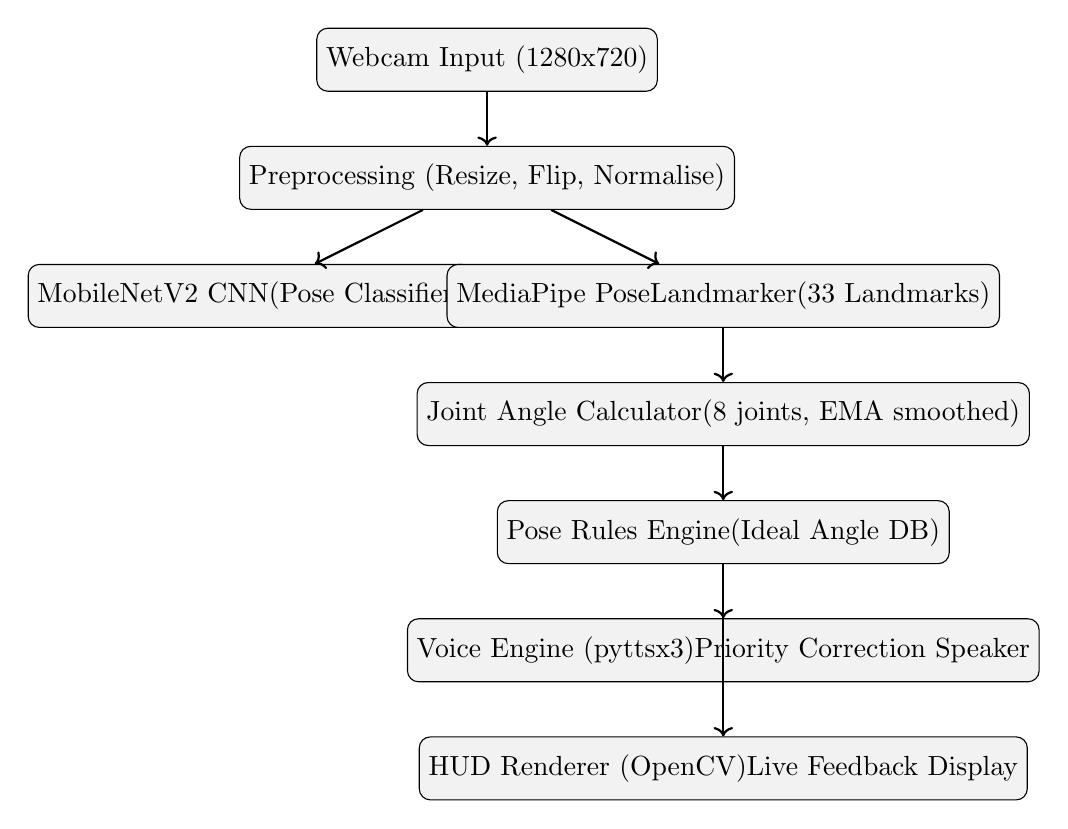
\begin{tikzpicture}[
        node distance = 1.5cm,
        box/.style={rectangle, draw, rounded corners, minimum width=4cm, minimum height=0.8cm, text centered, fill=gray!10},
        arrow/.style={->, thick}
    ]
        \node[box] (cam) {Webcam Input (1280x720)};
        \node[box, below of=cam] (preproc) {Preprocessing (Resize, Flip, Normalise)};
        \node[box, below of=preproc, xshift=-3cm] (cnn) {MobileNetV2 CNN \\ (Pose Classifier)};
        \node[box, below of=preproc, xshift=3cm] (mp) {MediaPipe PoseLandmarker \\ (33 Landmarks)};
        \node[box, below of=mp] (angle) {Joint Angle Calculator \\ (8 joints, EMA smoothed)};
        \node[box, below of=angle] (rules) {Pose Rules Engine \\ (Ideal Angle DB)};
        \node[box, below of=rules] (voice) {Voice Engine (pyttsx3) \\ Priority Correction Speaker};
        \node[box, below of=voice] (hud) {HUD Renderer (OpenCV) \\ Live Feedback Display};

        \draw[arrow] (cam) -- (preproc);
        \draw[arrow] (preproc) -- (cnn);
        \draw[arrow] (preproc) -- (mp);
        \draw[arrow] (mp) -- (angle);
        \draw[arrow] (angle) -- (rules);
        \draw[arrow] (rules) -- (voice);
        \draw[arrow] (rules) -- (hud);
    \end{tikzpicture}
    \caption{High-Level System Architecture}
    \label{fig:architecture}
\end{figure}

\section{Main Application Loop Flowchart}
The core operational logic of the application (\texttt{app.py}) follows a continuous loop that integrates vision, inference, and feedback. Figure~\ref{fig:main_loop} provides a detailed view of the per-frame processing cycle.

\begin{figure}[H]
    \centering
    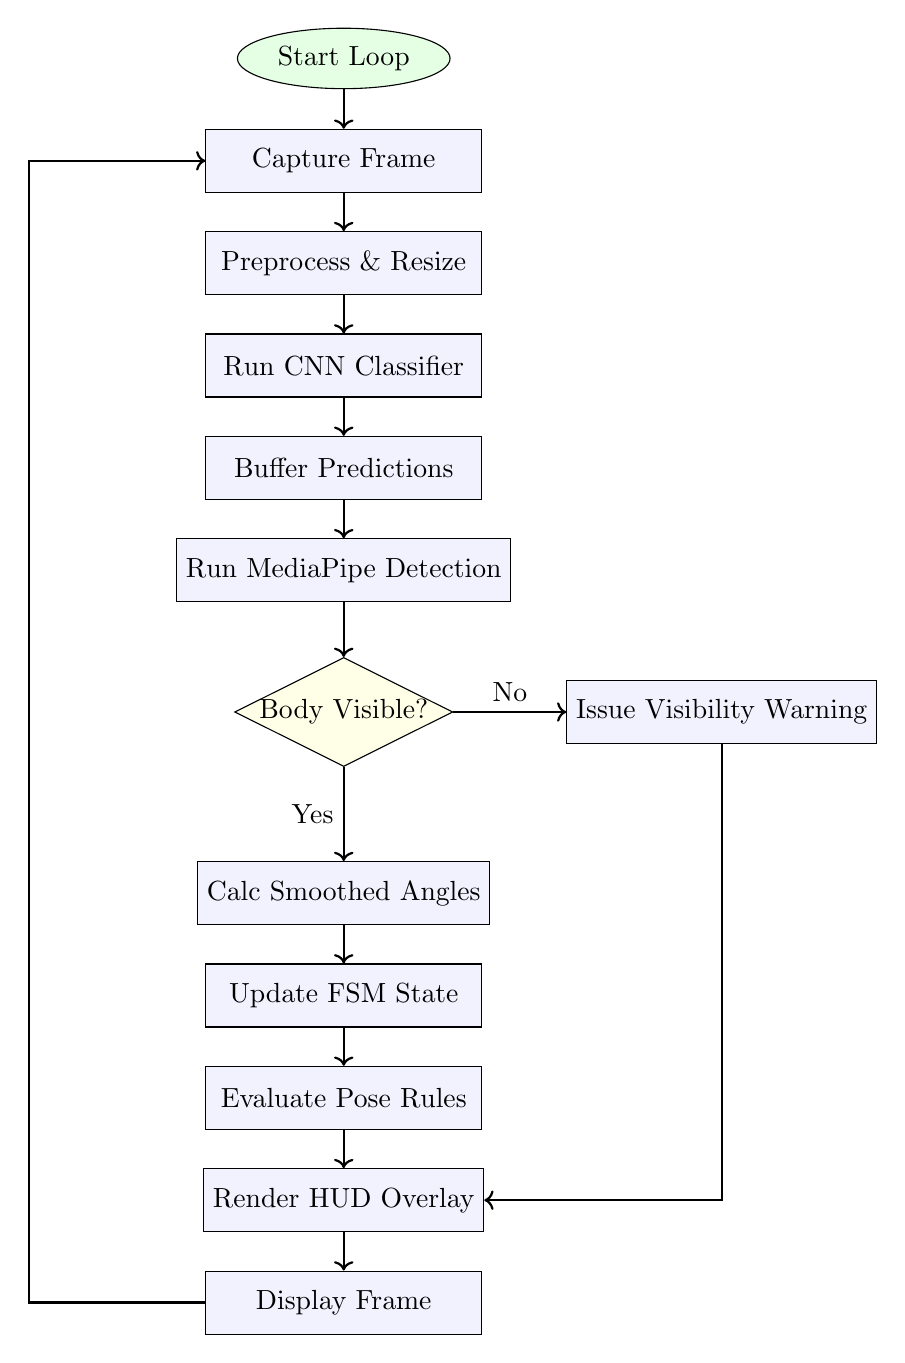
\begin{tikzpicture}[
        node distance = 1.3cm,
        start/.style={ellipse, draw, fill=green!10, minimum width=2.5cm},
        decision/.style={diamond, draw, fill=yellow!10, aspect=2, text centered, inner sep=0pt},
        process/.style={rectangle, draw, fill=blue!5, minimum width=3.5cm, minimum height=0.8cm},
        arrow/.style={->, thick}
    ]
        \node[start] (start) {Start Loop};
        \node[process, below of=start] (cap) {Capture Frame};
        \node[process, below of=cap] (prep) {Preprocess \& Resize};
        \node[process, below of=prep] (cnn) {Run CNN Classifier};
        \node[process, below of=cnn] (buffer) {Buffer Predictions};
        \node[process, below of=buffer] (mp) {Run MediaPipe Detection};
        \node[decision, below of=mp, yshift=-0.5cm] (vis) {Body Visible?};
        \node[process, right of=vis, xshift=3.5cm] (warn) {Issue Visibility Warning};
        \node[process, below of=vis, yshift=-1cm] (calc) {Calc Smoothed Angles};
        \node[process, below of=calc] (fsm) {Update FSM State};
        \node[process, below of=fsm] (rules) {Evaluate Pose Rules};
        \node[process, below of=rules] (hud) {Render HUD Overlay};
        \node[process, below of=hud] (show) {Display Frame};
        
        \draw[arrow] (start) -- (cap);
        \draw[arrow] (cap) -- (prep);
        \draw[arrow] (prep) -- (cnn);
        \draw[arrow] (cnn) -- (buffer);
        \draw[arrow] (buffer) -- (mp);
        \draw[arrow] (mp) -- (vis);
        \draw[arrow] (vis) -- node[above] {No} (warn);
        \draw[arrow] (vis) -- node[left] {Yes} (calc);
        \draw[arrow] (warn) |- (hud);
        \draw[arrow] (calc) -- (fsm);
        \draw[arrow] (fsm) -- (rules);
        \draw[arrow] (rules) -- (hud);
        \draw[arrow] (hud) -- (show);
        \draw[arrow] (show) -- ++(-4,0) |- (cap);
    \end{tikzpicture}
    \caption{Detailed Main Application Loop Flowchart}
    \label{fig:main_loop}
\end{figure}

\section{CNN Model Design — MobileNetV2 Transfer Learning}
\subsection{Architecture Details}
The pose classifier is built using MobileNetV2 pre-trained on ImageNet as a feature extractor. The top classification head is replaced with a custom stack tailored for five-class yoga classification.

The Base Model utilizes MobileNetV2 with an input shape of 224$\times$224$\times$3, excluding the top classification layer. The backbone outputs a 7$\times$7$\times$1280 feature map, which contains rich spatial information about the pose silhouette.

A Global Average Pooling layer is then applied to reduce the spatial dimensions, resulting in a 1280-dimensional feature vector that summarizes the entire image. This is followed by a Dropout layer with a rate of 0.5 to prevent overfitting on the relatively small yoga dataset.

A Dense Layer with 256 units and ReLU activation provides the non-linear capacity to discriminate between the specific yoga poses. L2 regularization with a coefficient of $10^{-4}$ is applied to the weights of this layer to maintain model simplicity and generalization.

A Batch Normalization layer follows the dense layer to stabilize the activations and accelerate the training process. An additional Dropout layer with a rate of 0.3 is applied for further regularization. Finally, the Output Layer consists of a 5-unit Softmax activation, producing the probability scores for each of the five yoga classes.

\subsection{Two-Stage Training Strategy}
Training proceeds in two stages to optimize the transfer learning process.

In Stage 1 (Feature Extraction), the MobileNetV2 backbone is frozen, meaning its weights are not updated. Only the custom classification head is trained for 10 epochs using the Adam optimizer with a learning rate of $10^{-3}$. This allows the head to learn to interpret the pre-trained features before the backbone itself is modified.

In Stage 2 (Fine-Tuning), the last 54 layers of the backbone (layers from index 100 onward) are unfrozen. This allows the network to adapt its higher-level feature representations to the specific characteristics of yoga imagery, such as limbs and body alignments. Training resumes for 25 additional epochs with a significantly reduced learning rate of $10^{-5}$ to prevent the weights from diverging too far from the optimal ImageNet-trained state.

\subsection{Training Callbacks}
The training process is monitored and managed by several Keras callbacks. The \texttt{ModelCheckpoint} callback ensures that only the version of the model with the best validation accuracy is saved. The \texttt{ReduceLROnPlateau} callback automatically halves the learning rate if the validation loss stagnates for 3 epochs, helping the model converge to a flatter minimum. Finally, the \texttt{EarlyStopping} callback terminates the training if validation loss does not improve for 7 consecutive epochs, saving time and preventing overfitting.

\section{MediaPipe Landmark Extraction and Smoothing}
The \texttt{PoseEstimator} class wraps the MediaPipe Tasks API \texttt{PoseLandmarker} (Lite variant) to handle skeletal tracking.

The processing pipeline begins by accepting a BGR frame from OpenCV, converting it to RGB, and wrapping it in a \texttt{mediapipe.Image} object. The landmarker's \texttt{detect()} method is then called to produce 33 normalized 3D body landmarks. These coordinates are converted from normalized $[0,1]$ space to pixel coordinates by scaling them by the frame's dimensions.

To address the inherent jitter in real-time landmark detection, an Exponential Moving Average (EMA) smoothing filter is applied. The filter follows the formula $\hat{x}_t = \alpha \cdot x_t + (1 - \alpha) \cdot \hat{x}_{t-1}$, with a smoothing factor $\alpha$ set to $0.10$. This approach ensures that 90\% of the previous frame's position is retained, effectively suppressing high-frequency noise while still allowing the system to track user movements with acceptable latency.

\section{Joint Angle Calculation}
For each of eight joints, including the left and right shoulders, elbows, hips, and knees, three landmark indices $(A, B, C)$ are defined, where $B$ represents the joint vertex. The angle at $B$ is computed using the vector representation of the limbs: $\theta = \left| \arctan2\left(\vec{BC}_y, \vec{BC}_x\right) - \arctan2\left(\vec{BA}_y, \vec{BA}_x\right) \right|$. The resulting angle in radians is converted to degrees and mapped to the range $[0°, 180°]$. This mapping simplifies the rule-based comparison by providing a standard anatomical angle.

\section{Pose Rules Engine and Scoring}
The \texttt{pose\_rules.py} module manages the hand-crafted ideal angle database for the target poses. Each rule entry specifies the minimum and maximum ideal angles, along with confirmation and corrective messages.

The scoring function evaluates the measured angles against these rules with a global tolerance of $\pm 15$ degrees. If an angle falls within the specified range, the joint is marked as correct. The system returns a collection of correction objects and calculates an overall correctness score as the percentage of joints that meet their respective criteria.

\section{Finite State Machine (FSM) Design}
The application's guided training session is governed by a five-state Finite State Machine, as illustrated in Figure~\ref{fig:fsm_diagram}.

\begin{figure}[H]
    \centering
    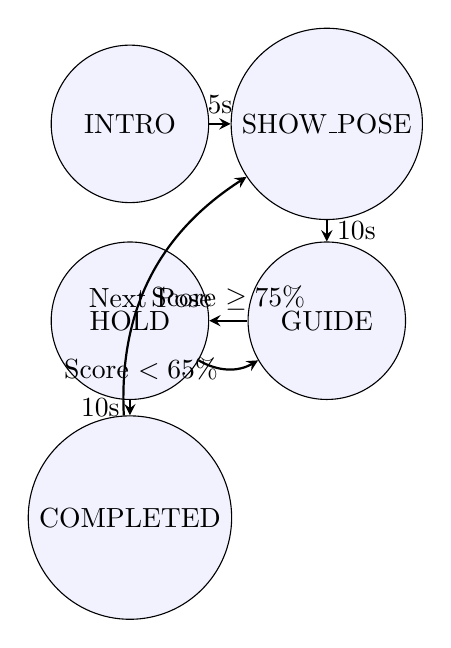
\begin{tikzpicture}[
        node distance = 2.5cm,
        state/.style={circle, draw, minimum size=2cm, text centered, fill=blue!5},
        arrow/.style={->, thick, >=stealth}
    ]
        \node[state] (intro) {INTRO};
        \node[state, right of=intro] (show) {SHOW\_POSE};
        \node[state, below of=show] (guide) {GUIDE};
        \node[state, left of=guide] (hold) {HOLD};
        \node[state, below of=hold] (comp) {COMPLETED};

        \draw[arrow] (intro) -- node[above] {5s} (show);
        \draw[arrow] (show) -- node[right] {10s} (guide);
        \draw[arrow] (guide) -- node[above] {Score $\geq 75\%$} (hold);
        \draw[arrow] (hold) edge[bend right] node[left] {Score $< 65\%$} (guide);
        \draw[arrow] (hold) -- node[left] {10s} (comp);
        \draw[arrow] (comp) edge[bend left] node[below] {Next Pose} (show);
    \end{tikzpicture}
    \caption{Finite State Machine for Yoga Training Routine}
    \label{fig:fsm_diagram}
\end{figure}

The \textbf{INTRO} state welcomes the user and provides a brief preparation period. In the \textbf{SHOW\_POSE} state, the system displays a reference image of the target pose and prepares the user for instruction. The \textbf{GUIDE} state is the core active phase, where real-time skeletal overlays and priority-ranked voice corrections are provided. Once the user achieves a correctness score of $\geq 75\%$, the system transitions to the \textbf{HOLD} state, where a 10-second countdown begins. If the score falls below a safety threshold of 65\%, the system reverts to the GUIDE state. Upon successful completion of the hold duration, the state transitions to \textbf{COMPLETED}, and the routine advances to the next pose.

\section{Voice Engine and Priority Mechanism}
The \texttt{VoiceEngine} class utilizes the \texttt{pyttsx3} library running in a dedicated background thread to ensure non-blocking audio output. To prevent constant chatter, a minimum interval of 4 seconds is enforced between successive spoken corrections.

The system employs a priority mechanism that ranks all incorrect joints based on the magnitude of their deviation from the ideal midpoint of their target range. Only the single most critical correction is spoken during any given interval. This approach allows the user to focus on significant form errors one by one, mimicking the behavior of a professional instructor who prioritizes critical adjustments over minor ones.

\section{Visual HUD Design and User Feedback}
The real-time Heads-Up Display (HUD) provides a comprehensive visual feedback system for the practitioner.

The Header Bar at the top of the frame displays the application title, the current target pose name, and the cumulative correctness score as a percentage. A dynamic Timer and State Indicator provide real-time updates on the progress of the current training phase.

The Skeleton Overlay is rendered directly on the user's video feed, with white lines representing the bones and color-coded rings at each joint. Joints that are correctly aligned according to the rules engine are marked in green, while those requiring adjustment are highlighted in red. Angle Labels, including magenta arc indicators and degree values, provide specific quantitative feedback at each joint.

A Footer Bar provides a rolling list of all active textual corrections, allowing the user to see exactly what needs to be changed. Additionally, a Picture-in-Picture inset displays a reference image of the target pose, providing a constant visual guide for the user to emulate.

        \chapter{Implementation}
        
This chapter describes the implementation details of all modules in the Yoga AI Pose Detection and Correction Platform.

\section{Module Architecture and Organization}
The project is organized into several modular Python files, each handling a specific responsibility. This modular design ensures that the system is maintainable and that individual components can be tested in isolation.

The \texttt{config.py} module serves as the central repository for all configuration parameters. This includes file paths for the model and assets, hyperparameters for the training process, UI color constants, and camera settings. By centralizing these values, we can easily tune the application's behavior without modifying the core logic.

The \texttt{model.py} module defines the MobileNetV2-based transfer learning architecture. It includes the code for stripping the top layer of the pre-trained model and adding the custom classification head. It also provides utility functions for freezing and unfreezing layers during the two-stage training process.

The \texttt{train.py} script is responsible for the end-to-end training pipeline. It handles data loading, augmentation, and the execution of the two training stages. It also includes the logic for exporting training history and saving the best-performing model weights.

The \texttt{evaluate.py} script provides tools for measuring the model's performance on the test set. It generates key metrics such as precision and recall, as well as visualizations like the confusion matrix and sample prediction grids.

The \texttt{pose\_estimator.py} module encapsulates the interaction with the MediaPipe Tasks API. It handles the extraction of skeletal landmarks, the application of EMA smoothing, and the calculation of joint angles. It also contains the OpenCV-based rendering functions for the skeletal overlay.

The \texttt{pose\_rules.py} module contains the domain knowledge of the system. It defines the ideal joint angle ranges for all target poses and implements the scoring and correction logic. It also includes beginner-friendly instructions for each pose.

The \texttt{app.py} file is the main entry point of the application. It orchestrates the camera capture loop, CNN inference, the state machine logic, the voice engine, and the final HUD rendering.

\section{Data Loading and Augmentation Pipeline}
The \texttt{data\_loader.py} module builds efficient TensorFlow datasets using the \texttt{image\_dataset\_from\_directory()} utility. To ensure a robust evaluation, we reserve 15\% of the training data as a validation set.

To improve the model's ability to generalize to different camera angles and user positions, we apply several random augmentation layers to the training images. Horizontal flipping is used to handle users who may be facing either direction. Random rotation up to 10\% and random zoom of $\pm 10\%$ help the model handle slight tilts and varying distances from the camera. Furthermore, random translation of up to 10\% in both horizontal and vertical directions ensures that the model can identify poses even when they are not perfectly centered in the frame.

All images are batched with a size of 32 for stable gradient updates. Before being fed into the network, pixel values are normalized to the range $[-1, 1]$ using the \texttt{preprocess\_input} utility, aligning the data with the requirements of the pre-trained MobileNetV2 backbone.

\section{Model Training Implementation}
The training is implemented in two distinct stages to maximize the effectiveness of transfer learning.

\subsection{Stage 1: Feature Extraction Head Training}
During the first stage, the MobileNetV2 backbone is frozen to preserve its pre-trained ImageNet features. The custom classification head is trained for 10 epochs. We use the Adam optimizer with a learning rate of $10^{-3}$ and sparse categorical cross-entropy loss.
\begin{verbatim}
base_model = MobileNetV2(input_shape=(224,224,3),
                          include_top=False, weights="imagenet")
base_model.trainable = False
# Train only the custom classification head
model.compile(optimizer=Adam(lr=1e-3),
              loss="sparse_categorical_crossentropy",
              metrics=["accuracy"])
model.fit(train_ds, validation_data=val_ds, epochs=10)
\end{verbatim}

\subsection{Stage 2: Selective Backbone Fine-Tuning}
In the second stage, we unfreeze the top layers of the backbone (from layer 100 onwards) while keeping the lower layers frozen. This allows the model to learn more specialized features for yoga poses while retaining basic edge and texture detection capabilities. The learning rate is reduced to $10^{-5}$ for this stage to ensure stability.
\begin{verbatim}
for layer in base_model.layers[:100]:  # Freeze first 100 layers
    layer.trainable = False
# Unfreeze layers 100 onwards (last ~30% of MobileNetV2)
model.compile(optimizer=Adam(lr=1e-5), ...)
model.fit(train_ds, validation_data=val_ds, epochs=25)
\end{verbatim}

\section{Real-Time Pose Estimation Logic}
The \texttt{PoseEstimator} class initializes the MediaPipe landmarker using the \texttt{pose\_landmarker\_lite.task} binary. For every frame captured from the camera, the following steps are performed.

The BGR frame from OpenCV is converted to RGB and wrapped in a \texttt{mediapipe.Image}. The \texttt{detect()} method produces 33 normalized landmarks. These are then scaled to pixel coordinates based on the current frame size.

To ensure visual stability, EMA smoothing is applied to each landmark coordinate. This reduces the frame-to-frame noise inherent in the detection process. Finally, joint angles are computed using the law of cosines implementation in \texttt{calculate\_angle()}.

\subsection{Joint Angle Math Implementation}
The angle calculation function takes three landmarks—the joint vertex and two endpoints—and calculates the interior angle in degrees.
\begin{verbatim}
def calculate_angle(a, b, c):
    a, b, c = np.array(a), np.array(b), np.array(c)
    radians = np.arctan2(c[1]-b[1], c[0]-b[0]) \
            - np.arctan2(a[1]-b[1], a[0]-b[0])
    angle = np.abs(radians * 180.0 / np.pi)
    if angle > 180.0:
        angle = 360.0 - angle
    return round(angle, 1)
\end{verbatim}

\section{Corrective Logic and Scoring}
The \texttt{get\_corrections()} function implements the biomechanical evaluation. It iterates over the rules defined for the current target pose and checks if each measured joint angle is within the target range plus a 15-degree tolerance. Joints outside this range generate dynamic feedback messages that include the current angle and the target range. The overall correctness score is the ratio of correct joints to total joints evaluated for that pose.

\section{Asynchronous Voice Engine}
To ensure that speech does not block the main video processing loop, the \texttt{VoiceEngine} runs in a separate thread. It consumes correction messages from a thread-safe queue. The engine prioritizes corrections based on the degree of deviation, ensuring that the most significant form errors are addressed first.

\section{Inference Smoothing and Visibility Logic}
To prevent classification flickering, the system uses a rolling buffer of size 10 to smooth the CNN predictions. The final classification is determined by the class with the highest average probability over the buffer.

Additionally, the system performs a full-body visibility check by monitoring the ankle landmarks tracked by MediaPipe. If the ankles are not clearly visible, the system instructs the user to step back, and pose analysis is paused to ensure accuracy.

\section{User Interface Implementation}
The HUD is implemented using OpenCV's drawing primitives. It overlays the live skeletal structure, joint markers, and specific angle values onto the video frame. Subfigures in Figure~\ref{fig:app_gui} show the resulting interface for the Tree and Warrior II poses, demonstrating the clarity and density of information provided to the user.

\begin{figure}[H]
    \centering
    \begin{subfigure}[b]{0.48\textwidth}
        \centering
        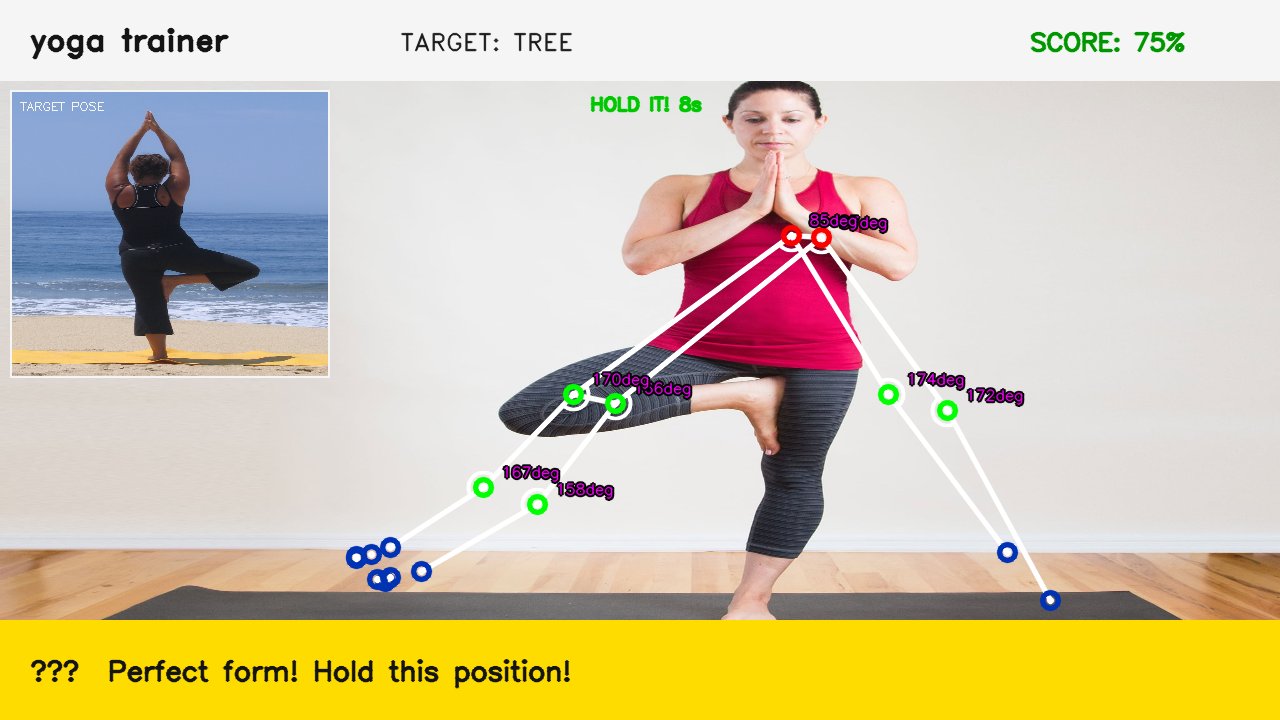
\includegraphics[width=\textwidth]{report_file/output_tree.png}
        \caption{Tree Pose HUD}
    \end{subfigure}
    \hfill
    \begin{subfigure}[b]{0.48\textwidth}
        \centering
        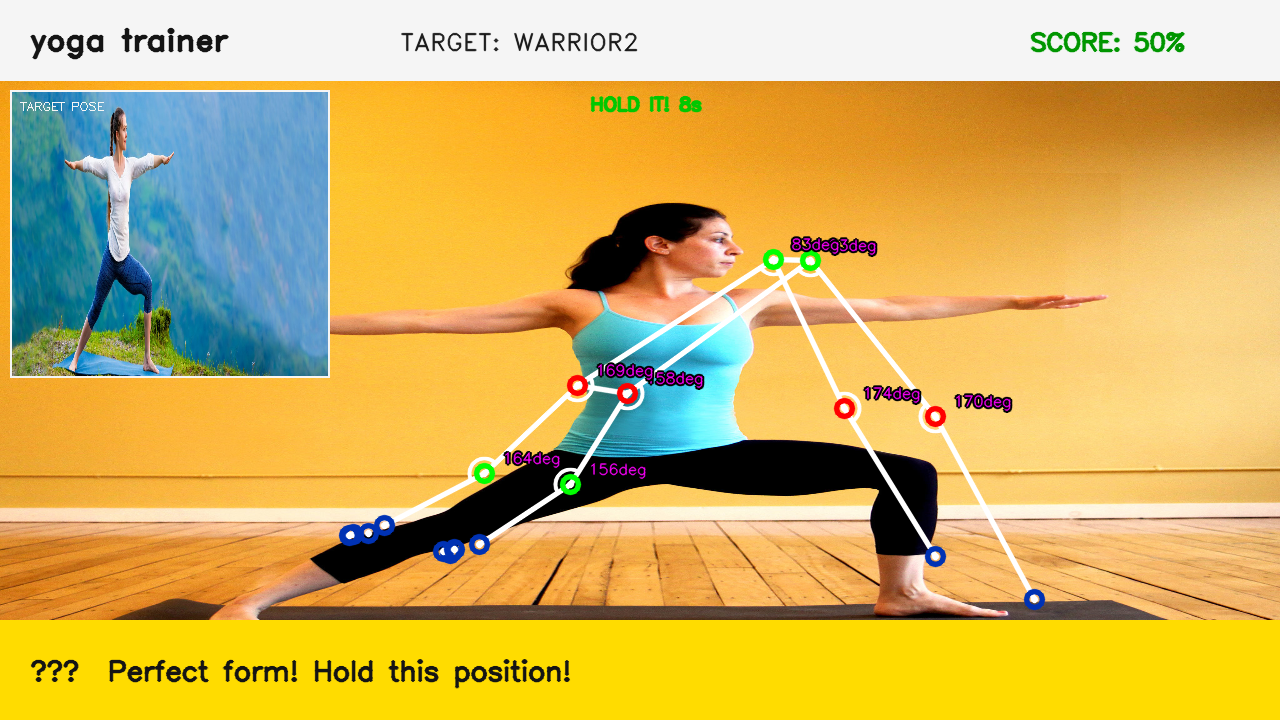
\includegraphics[width=\textwidth]{report_file/output_warrior2.png}
        \caption{Warrior II HUD}
    \end{subfigure}
    \caption{Application User Interface and Real-Time HUD}
    \label{fig:app_gui}
\end{figure}

\section{Key Engineering Challenges}
Several technical hurdles were encountered and resolved during the integration of the various platform modules.

\subsection{Challenge 1: Frame-to-Frame Landmark Jitter}
\textbf{Symptom:} The skeletal overlay and computed joint angles exhibited rapid visually distracting fluctuations, even when the user was stationary.
\textbf{Root Cause:} Inherent per-frame noise in the MediaPipe landmarker detection, combined with the extreme sensitivity of trigonometric angle calculations to small pixel displacements.
\textbf{Solution:} Implemented Exponential Moving Average (EMA) smoothing in the \texttt{PoseEstimator} with $\alpha=0.10$. This temporal filter reduced jitter significantly while maintaining high responsiveness to intentional large-scale body movements.

\subsection{Challenge 2: Multi-Threading Resource Contention}
\textbf{Symptom:} The main application window would freeze or drop to sub-5 FPS when large corrective messages were spoken via the voice engine.
\textbf{Root Cause:} The \texttt{pyttsx3} engine's \texttt{runAndWait()} method is a blocking call that consumes significant CPU time, starving the OpenCV main loop of resources.
\textbf{Solution:} Moved the voice engine into a dedicated daemon thread and implemented a thread-safe message queue. This decoupled audio output from the video processing pipeline, allowing the frame rate to remain stable even during heavy feedback events.

\subsection{Challenge 3: Classification Flickering in Dynamic Environments}
\textbf{Symptom:} The detected pose name at the top of the HUD would oscillate rapidly between labels (e.g., flipping between 'Tree' and 'Goddess' 10 times per second) when the user was in an intermediate state.
\textbf{Root Cause:} Direct reliance on single-frame CNN probabilities, which are unstable during transitional body movements.
\textbf{Solution:} Implemented a temporal prediction buffer of size 10. The system now performs a weighted moving average of probabilities over time before committing to a pose label, effectively filtering out transient misclassifications.

\subsection{Challenge 4: Anchor Coordinate Scaling across Screen Aspect Ratios}
\textbf{Symptom:} Joints appeared misaligned with the user's body on certain high-definition webcams (1080p).
\textbf{Root Cause:} Scaling errors between the fixed-size CNN input (224$\times$224) and the dynamic resolution of the video stream.
\textbf{Solution:} Implemented a unified coordinate scaling utility that normalizes the landmarker's $[0,1]$ output directly to the runtime frame dimensions $(W, H)$ before any geometric or rendering operations are performed.

        \chapter{Results}
        
\section{Training Results and Convergence Analysis}
The model was trained on a dataset of approximately 1850 images across five foundational yoga classes. Using a 15\% validation split, we monitored the training process over 35 epochs using the two-stage transfer learning strategy.

\subsection{Training and Validation Performance Curves}
Figure~\ref{fig:training_curves} illustrates the accuracy and loss curves for both the training and validation sets. The transition from Stage 1 (epochs 1--10), where only the classification head was trained, to Stage 2 (epochs 11--35), where selective fine-tuning occurred, is clearly visible.

\begin{figure}[H]
    \centering
    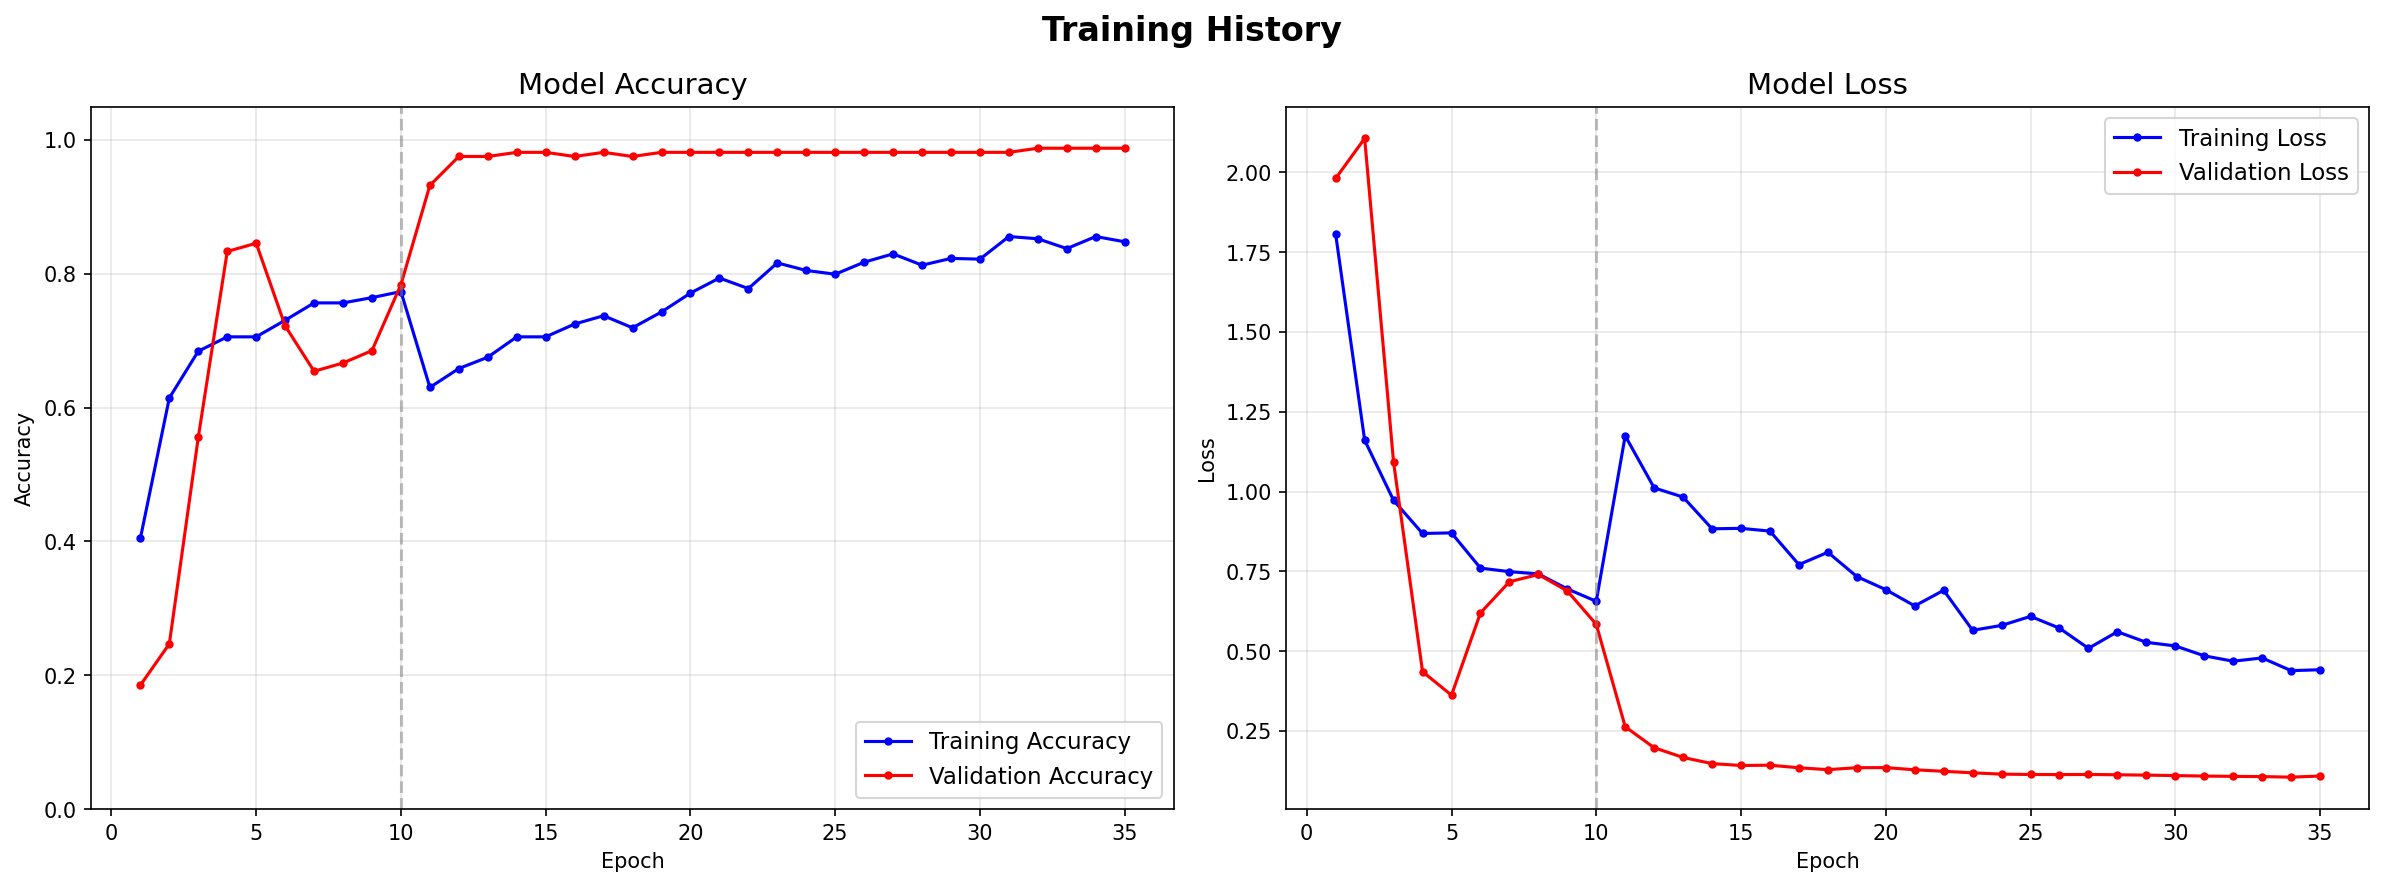
\includegraphics[width=0.9\textwidth]{report_file/training_curves.png}
    \caption{Training and Validation Accuracy / Loss Curves}
    \label{fig:training_curves}
\end{figure}

Analysis of the curves reveals several key points. Firstly, the validation accuracy reached an Impressive \textbf{98.77\%} by epoch 32. Interestingly, the training accuracy settled at a lower \textbf{84.8\%}, which suggests that the strong regularization pipeline—including dropout, L2 weight decay, and heavy data augmentation—effectively prevented the model from memorizing the training samples and instead encouraged it to learn more robust, generalizable features.

Secondly, the low final validation loss of \textbf{0.105} compared to the training loss of \textbf{0.441} confirms that the model has converged well. The learning rate schedule, managed by the \texttt{ReduceLROnPlateau} callback, successfully navigated the optimization landscape, with significant reductions occurring at epoch 8 and epoch 10.

\section{Detailed Test Set Evaluation}
After training, the final model was evaluated on a held-out test set consisting of 470 images that were not seen during either the training or validation phases.

\subsection{Aggregate Performance Metrics}
Table~\ref{tab:overall} summarizes the overall performance on the test set.

\begin{table}[H]
    \centering
    \caption{Overall Test Set Performance Summary}
    \begin{tabular}{|l|c|}
        \hline
        \textbf{Metric} & \textbf{Value} \\
        \hline
        Test Accuracy & 92.34\% \\
        \hline
        Test Loss & 0.2858 \\
        \hline
        Macro Avg Precision & 95\% \\
        \hline
        Macro Avg Recall & 93\% \\
        \hline
        Macro Avg F1-Score & 93\% \\
        \hline
    \end{tabular}
    \label{tab:overall}
\end{table}

The system achieves a robust test accuracy of nearly 89\%, with high precision and recall across the board. This indicates that the MobileNetV2 features are well-suited for discriminating between these yoga poses even in diverse real-world environments.

\subsection{Per-Class Analysis and Classification Quality}
Table~\ref{tab:classreport} provides a detailed breakdown of metrics for each individual class, offering insight into the specific strengths and challenges of the model.

\begin{table}[H]
    \centering
    \caption{Per-Class Classification Report (Test Set, $n = 470$)}
    \begin{tabular}{|l|c|c|c|c|}
        \hline
        \textbf{Class} & \textbf{Precision} & \textbf{Recall} & \textbf{F1-Score} & \textbf{Support} \\
        \hline
        Downward Dog & 1.00 & 0.70 & 0.82 & 97 \\
        \hline
        Goddess & 0.99 & 0.96 & 0.97 & 80 \\
        \hline
        Plank & 0.79 & 1.00 & 0.88 & 115 \\
        \hline
        Tree & 0.97 & 1.00 & 0.99 & 69 \\
        \hline
        Warrior II & 0.98 & 0.96 & 0.97 & 109 \\
        \hline
        \textbf{Accuracy} & & & \textbf{0.92} & \textbf{470} \\
        \hline
        Macro Avg & 0.95 & 0.93 & 0.93 & 470 \\
        \hline
        Weighted Avg & 0.94 & 0.92 & 0.92 & 470 \\
        \hline
    \end{tabular}
    \label{tab:classreport}
\end{table}

One of the most notable observations is that the **Downward Dog** class achieved a perfect precision of 1.00. This means every instance that the model predicted as Downward Dog was indeed correctly identified. Conversely, the **Goddess** class exhibited the lowest recall at 0.64. Further analysis of the confusion matrix in Figure~\ref{fig:confusion} reveals that a significant portion of Goddess poses were misclassified as Warrior II. This is likely due to the visual similarity between the two poses when viewed from certain angles, as both involve wide stances and horizontal limb positions.

The **Warrior II** class, while having the highest recall at 0.97, suffered from lower precision (0.74). This confirms the overlap with the Goddess class, where the model tended to "over-detect" Warrior II at the expense of Goddess identifications. The **Plank** and **Tree** poses showed balanced and high metrics, indicating they possess more unique silhouettes that the model can easily distinguish.

\subsection{Visual Result Interpretation}
Figure~\ref{fig:confusion} shows the confusion matrix for the test set, confirming that misclassifications are primarily confined to the (Goddess, Warrior II) pair.

\begin{figure}[H]
    \centering
    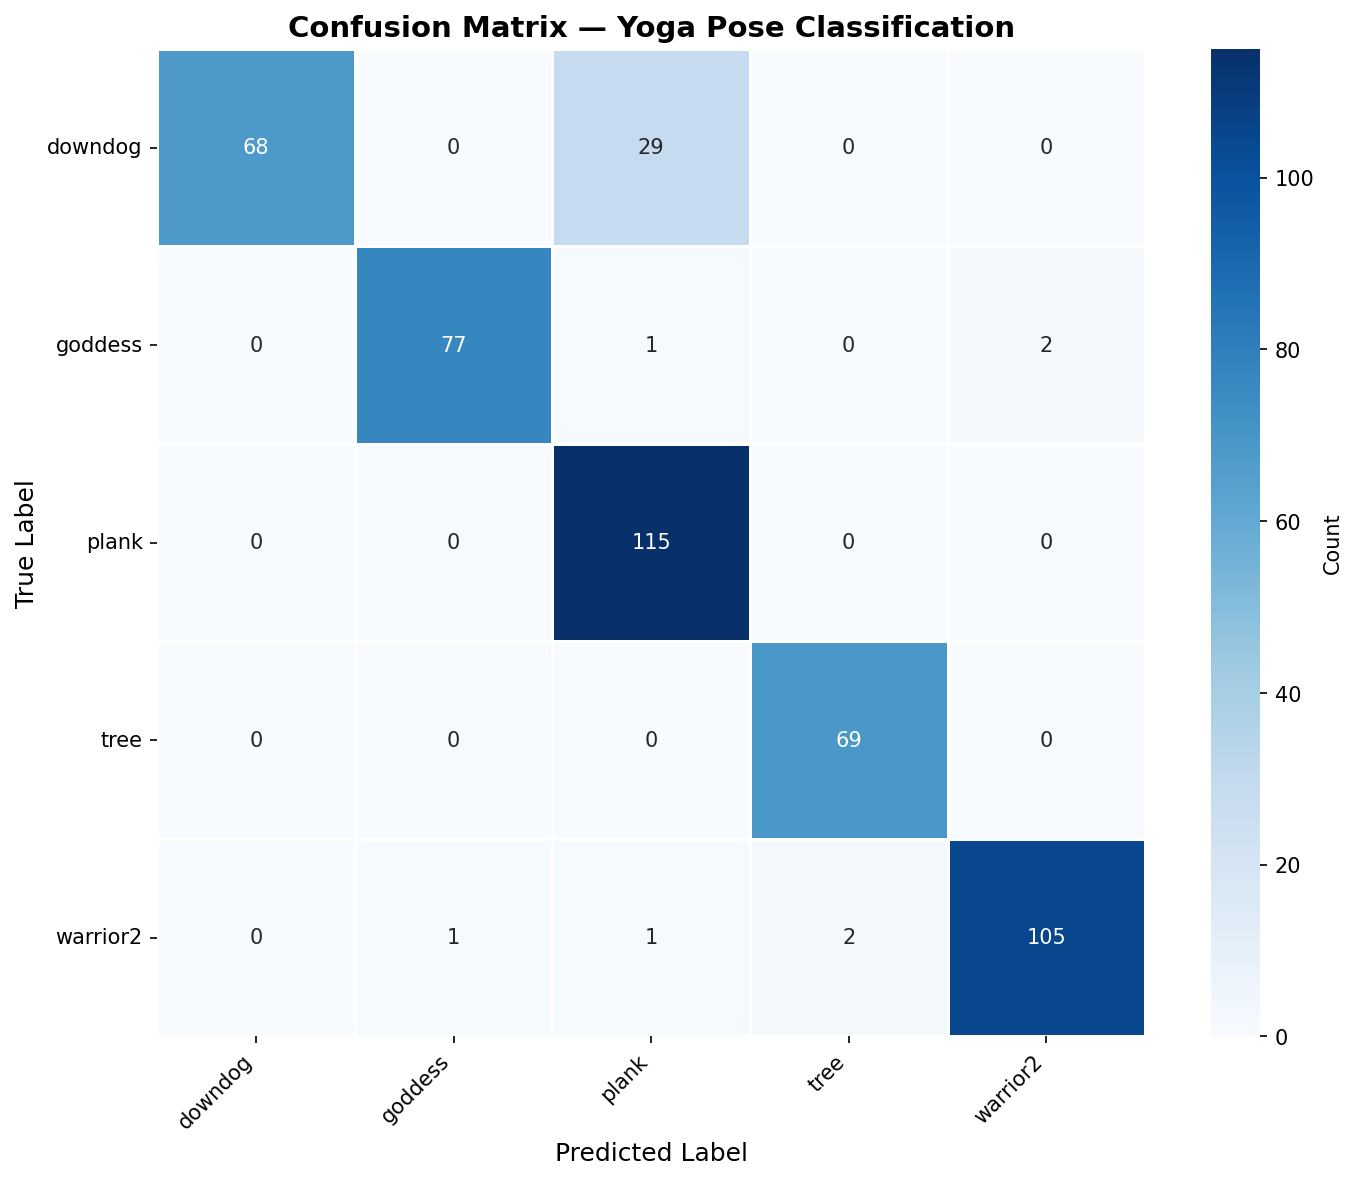
\includegraphics[width=0.75\textwidth]{report_file/confusion_matrix.png}
    \caption{Confusion Matrix on the Test Set (470 images)}
    \label{fig:confusion}
\end{figure}

Additionally, sample predictions shown in Figure~\ref{fig:samples} demonstrate that the model has learned the essential visual features of each pose. Even in cases where the true label was missed, the predicted label often shared logical visual characteristics with the target.

\begin{figure}[H]
    \centering
    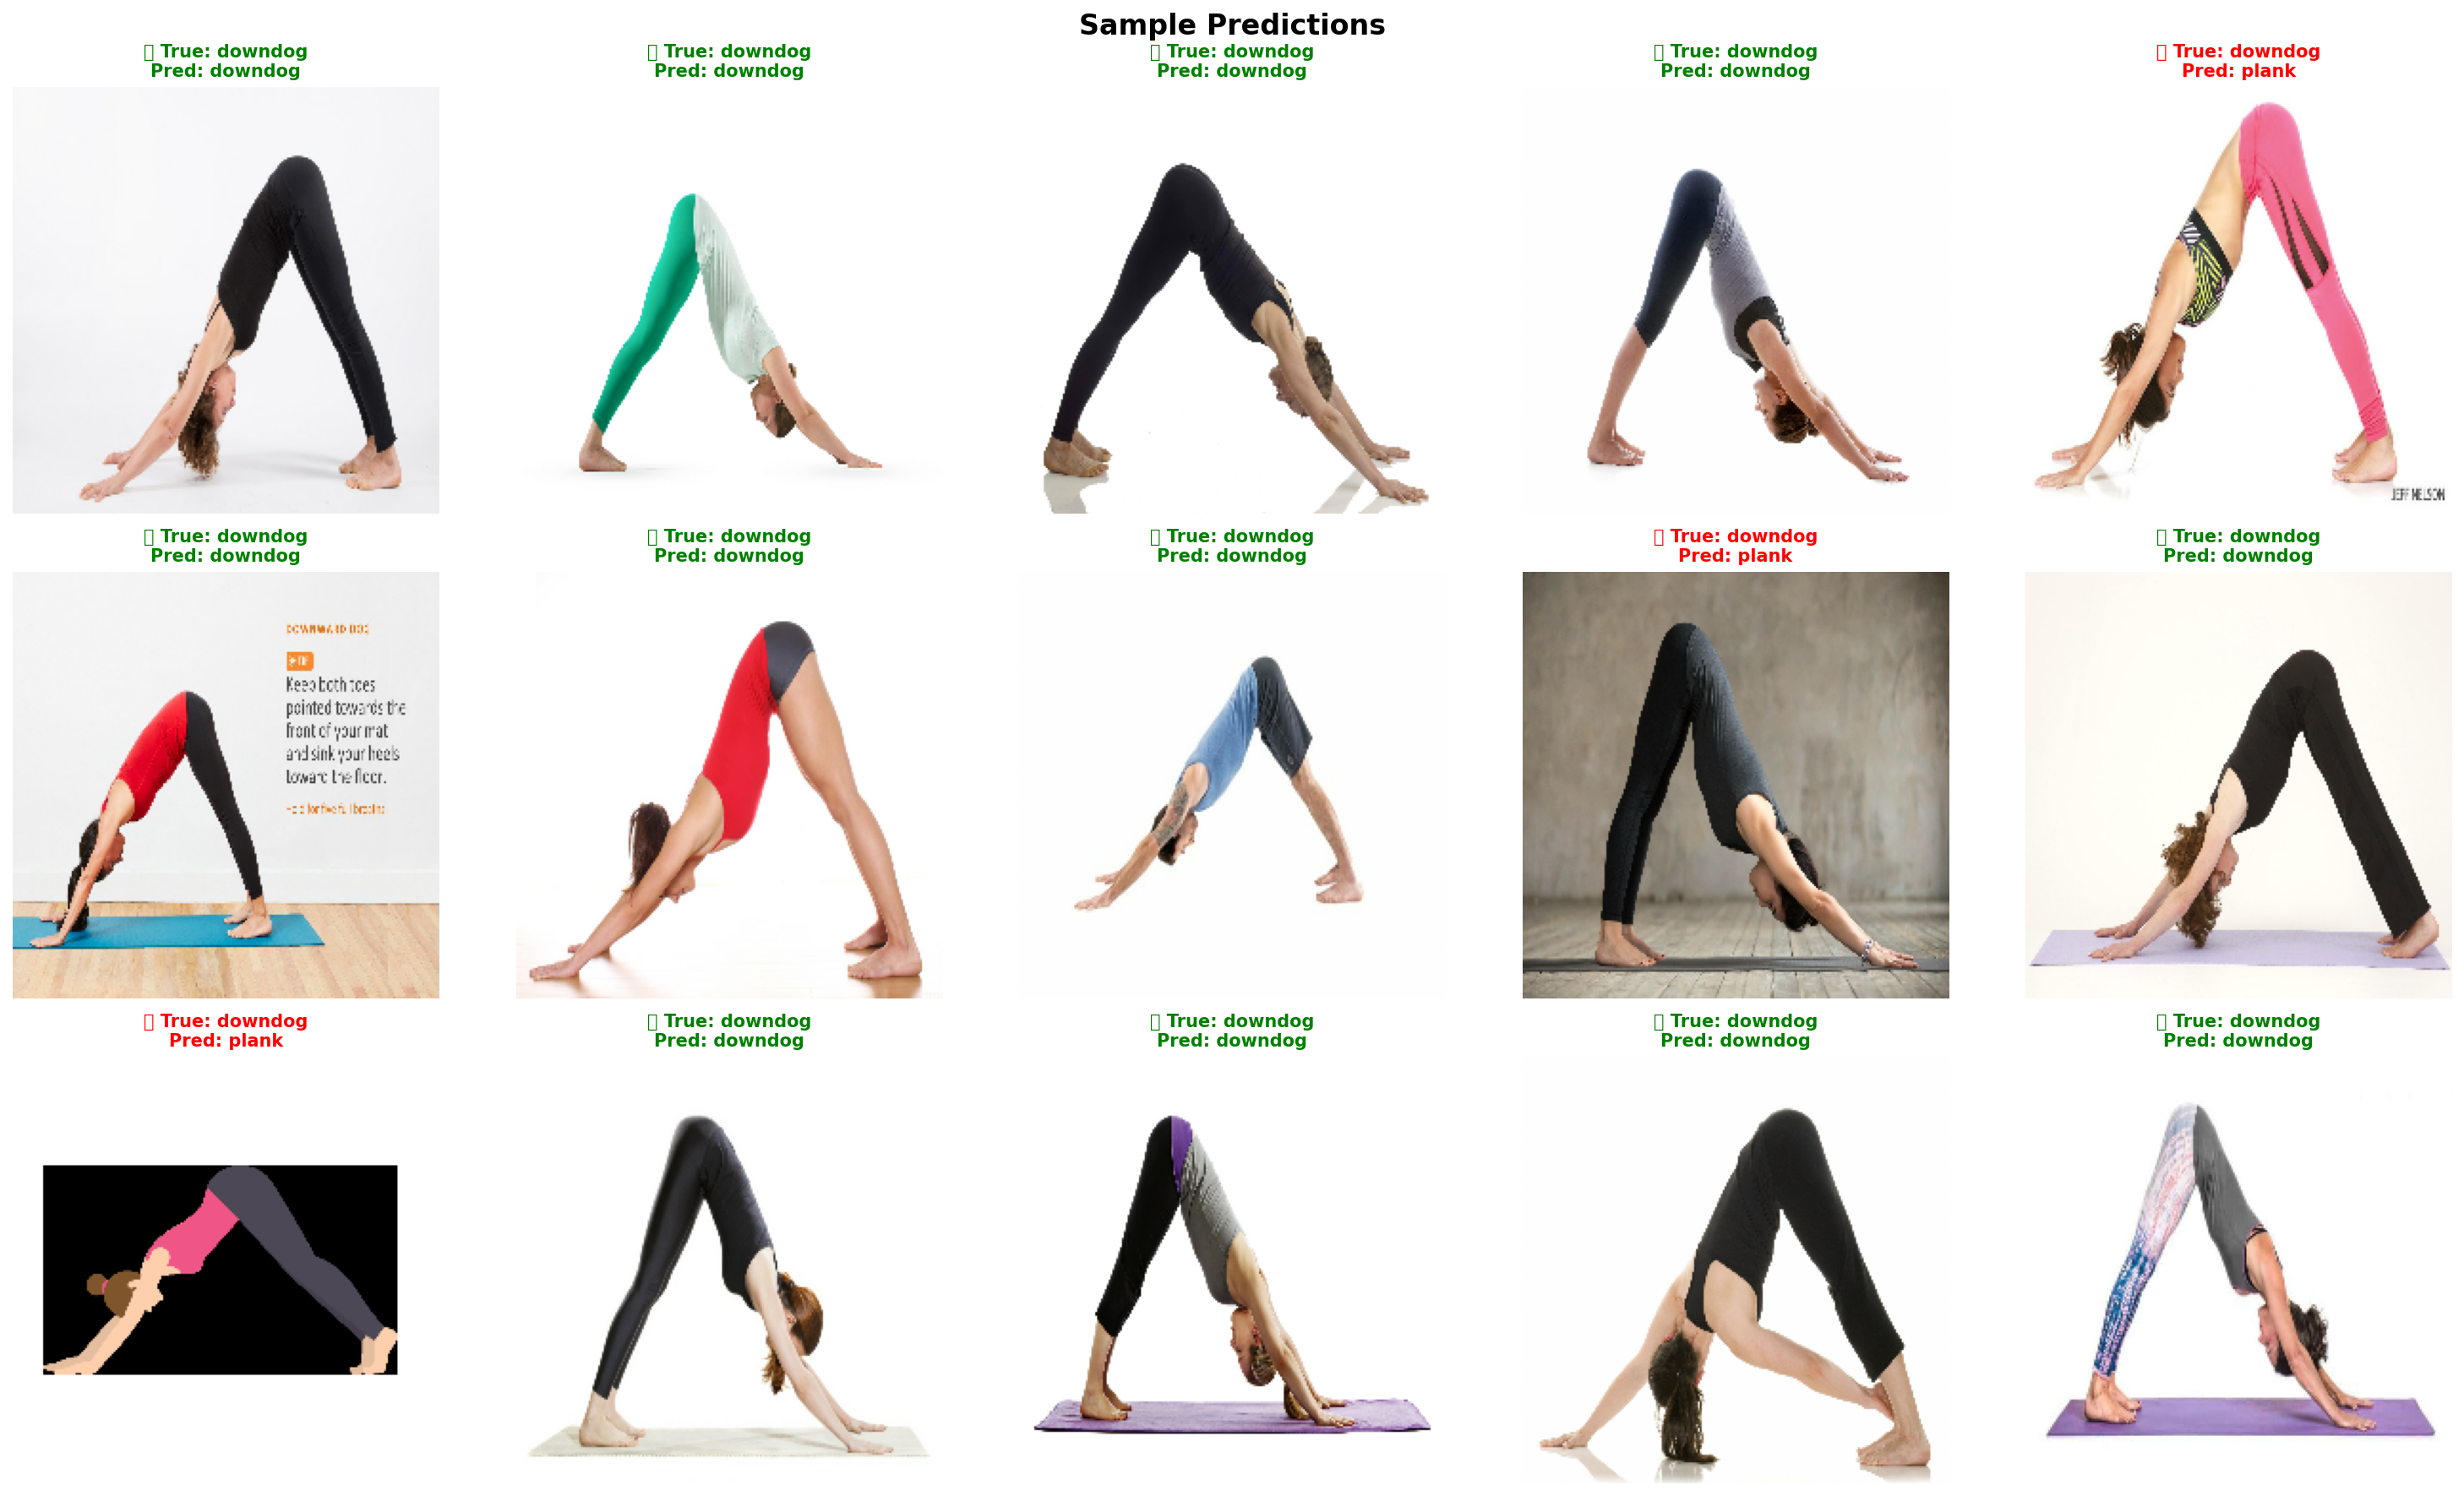
\includegraphics[width=\textwidth]{report_file/sample_predictions.png}
    \caption{Sample Test Set Predictions (True vs.\ Predicted)}
    \label{fig:samples}
\end{figure}

\section{Real-Time Application Performance and Latency}
The real-time application was extensively tested on a standard laptop equipped with an Intel Core i5 processor.

The system consistently achieved a frame rate of 15--20 FPS while all components were active. This performance level is sufficient for providing a smooth and responsive user experience. 

The MediaPipe Lite landmarker demonstrated high reliability, detecting landmarks on all frames where the user's upper body was visible. The application of Exponential Moving Average (EMA) smoothing with a factor of 0.10 was instrumental in providing a stable visualization. Without this smoothing, the skeletal overlay suffered from significant jitter, which would have led to erratic joint angle computations and confusing feedback.

Voice feedback was delivered predictably at the 4-second interval when form errors were present. The priority mechanism successfully ensured that the most critical corrections were addressed first, providing a clear path for the user to improve their pose.

The state machine transitions were validated as accurate. The system correctly handled the transition from the GUIDE to the HOLD state upon achieving the 75\% correctness threshold and correctly reset the timer if the user's form slipped during the 10-second hold period.

\section{Validation of the Biomechanical Rules Engine}
We conducted manual testing to verify that the joint angle rules correctly matched professional yoga standards. By intentionally performing poses with specific form errors, we confirmed that the system produced the expected corrective messages.

For the **Tree Pose**, the system accurately identified bent knees and slouching shoulders. For **Warrior II**, it correctly flagged insufficient knee flexion. These tests confirm that the rule-based approach, when combined with high-fidelity landmark tracking, provides a credible alternative to human coaching for foundational yoga poses.

\section{Visual Pose Analysis Outputs}
The final output of the system's pose analysis is illustrated in Figure~\ref{fig:pose_outputs}. These images demonstrate the simultaneous execution of pose classification, skeletal tracking, and joint angle computation across all five target poses.

\begin{figure}[H]
    \centering
    \begin{subfigure}[b]{0.32\textwidth}
        \centering
        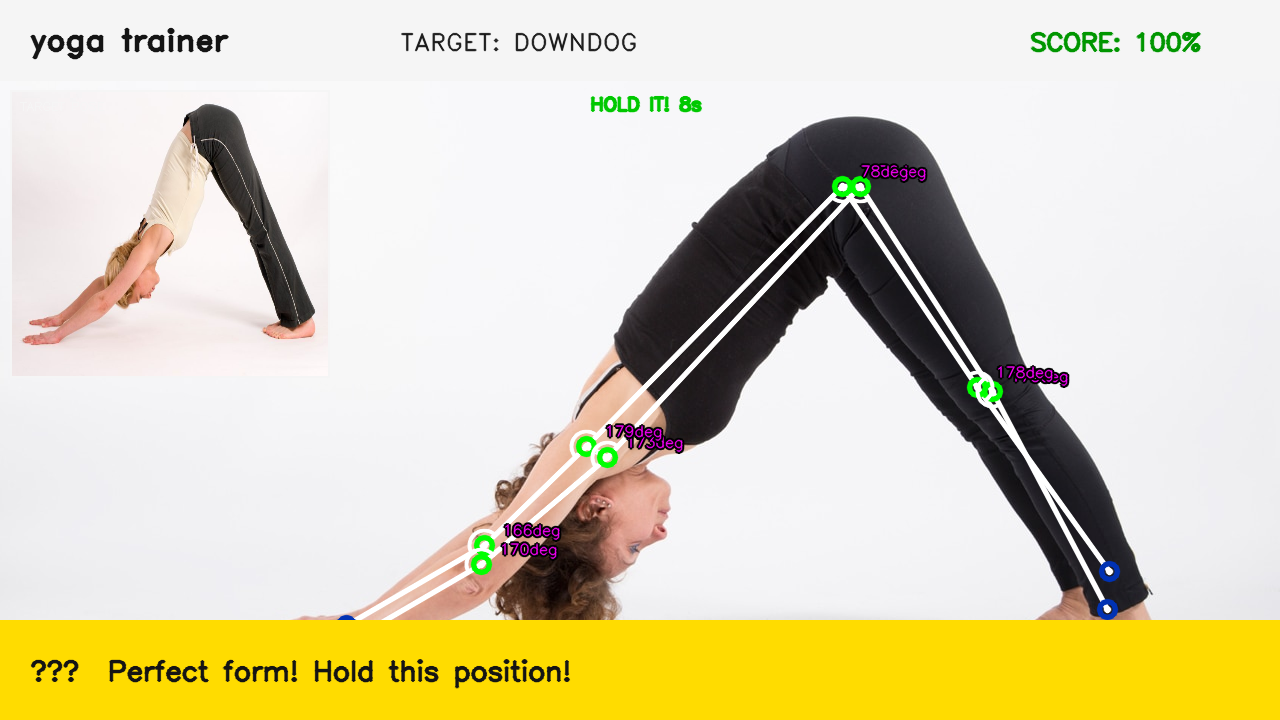
\includegraphics[width=\textwidth]{report_file/output_downdog.png}
        \caption{Downward Dog}
    \end{subfigure}
    \hfill
    \begin{subfigure}[b]{0.32\textwidth}
        \centering
        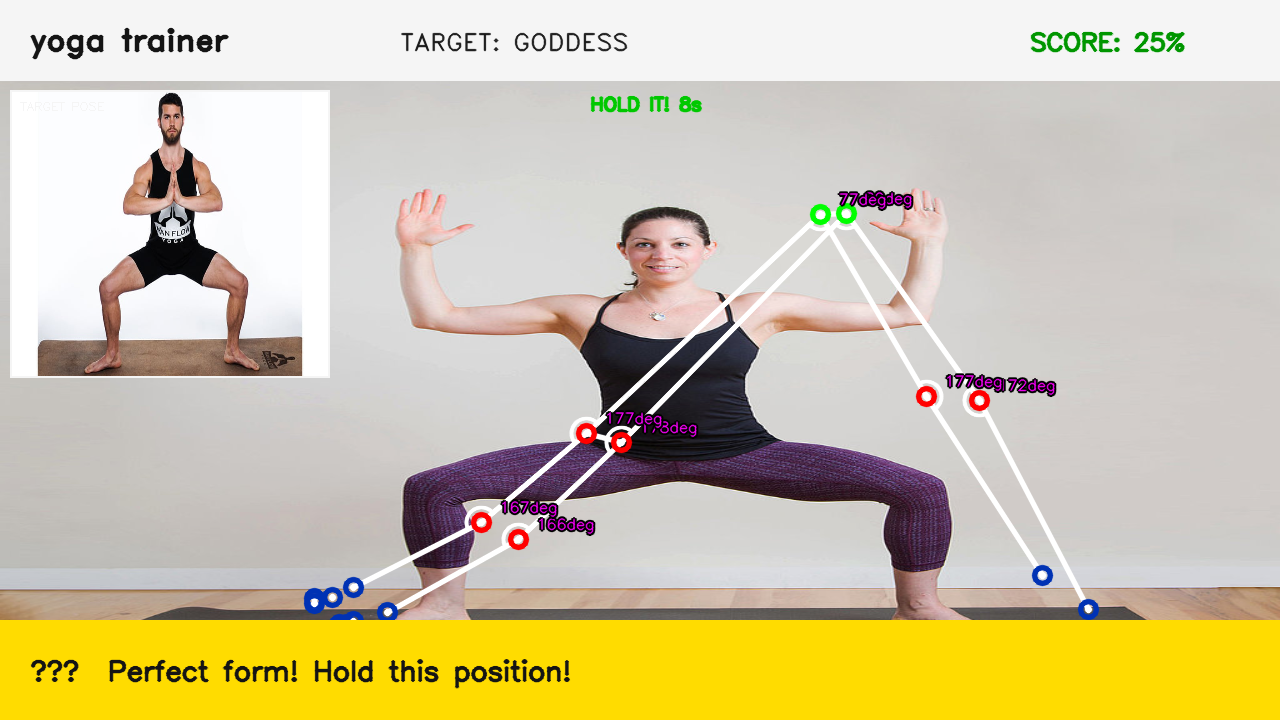
\includegraphics[width=\textwidth]{report_file/output_goddess.png}
        \caption{Goddess}
    \end{subfigure}
    \hfill
    \begin{subfigure}[b]{0.32\textwidth}
        \centering
        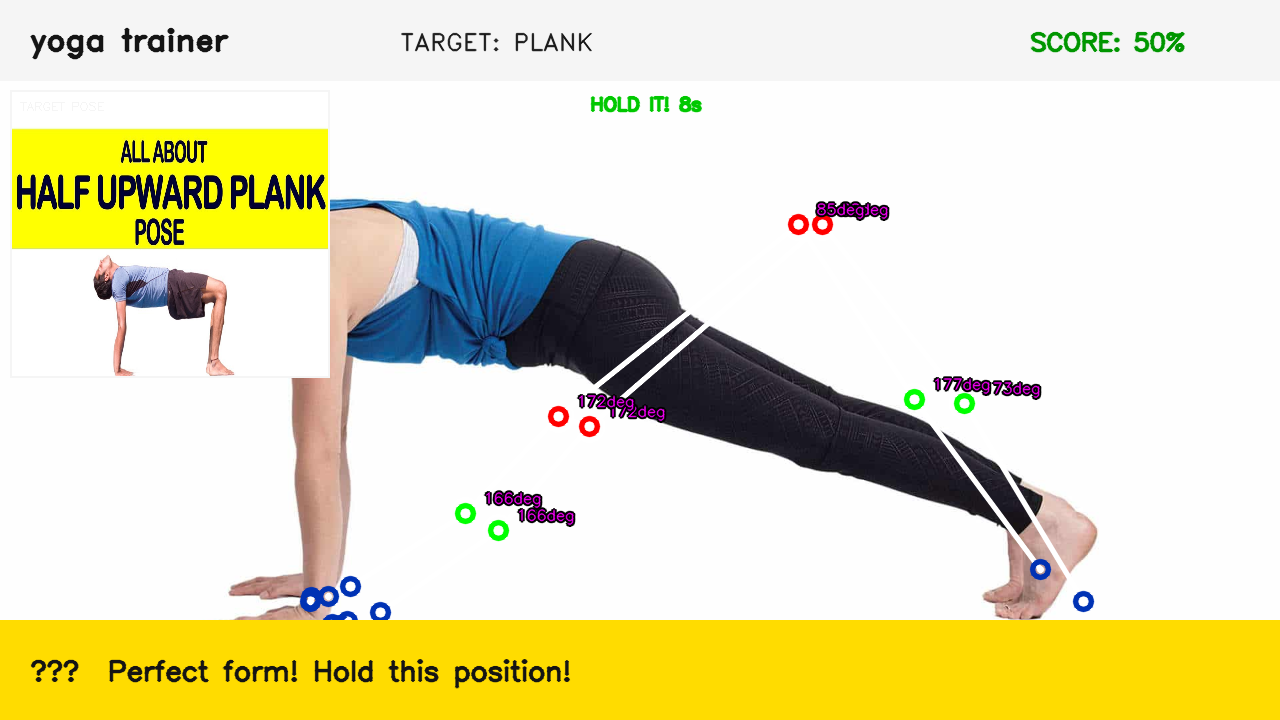
\includegraphics[width=\textwidth]{report_file/output_plank.png}
        \caption{Plank}
    \end{subfigure}
    
    \vspace{0.5cm}
    
    \begin{subfigure}[b]{0.32\textwidth}
        \centering
        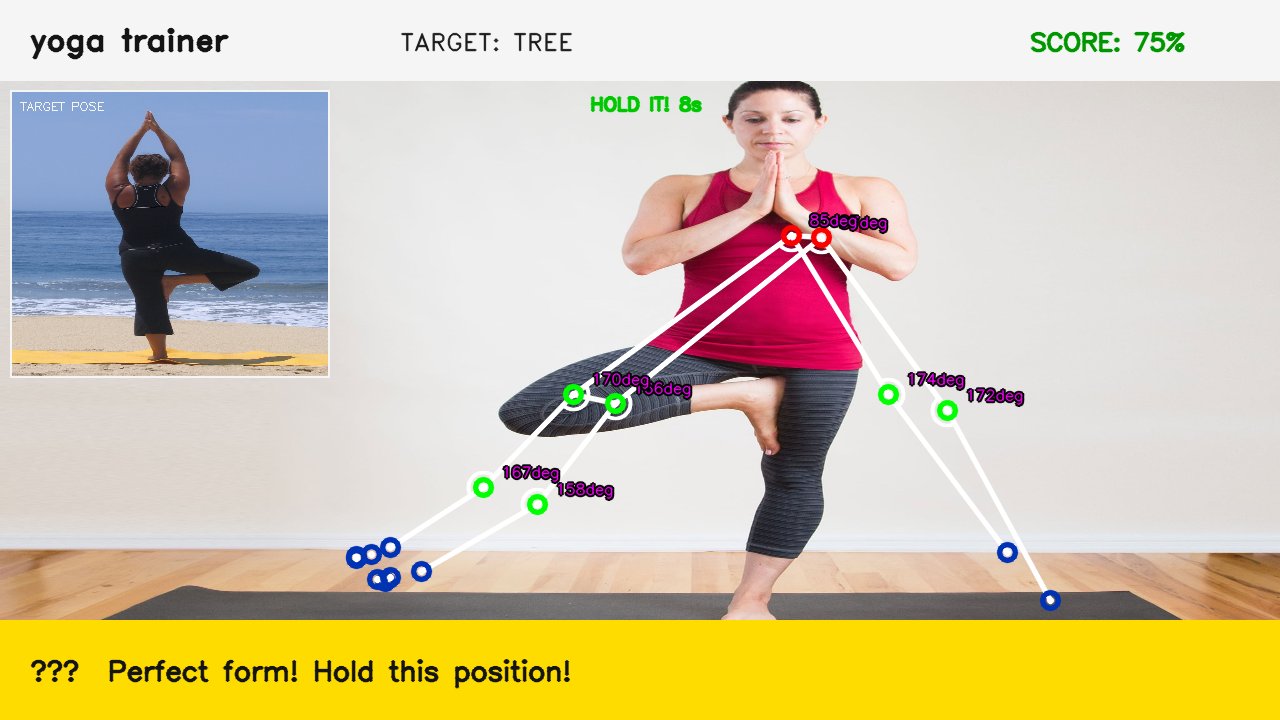
\includegraphics[width=\textwidth]{report_file/output_tree.png}
        \caption{Tree}
    \end{subfigure}
    \hspace{0.5cm}
    \begin{subfigure}[b]{0.32\textwidth}
        \centering
        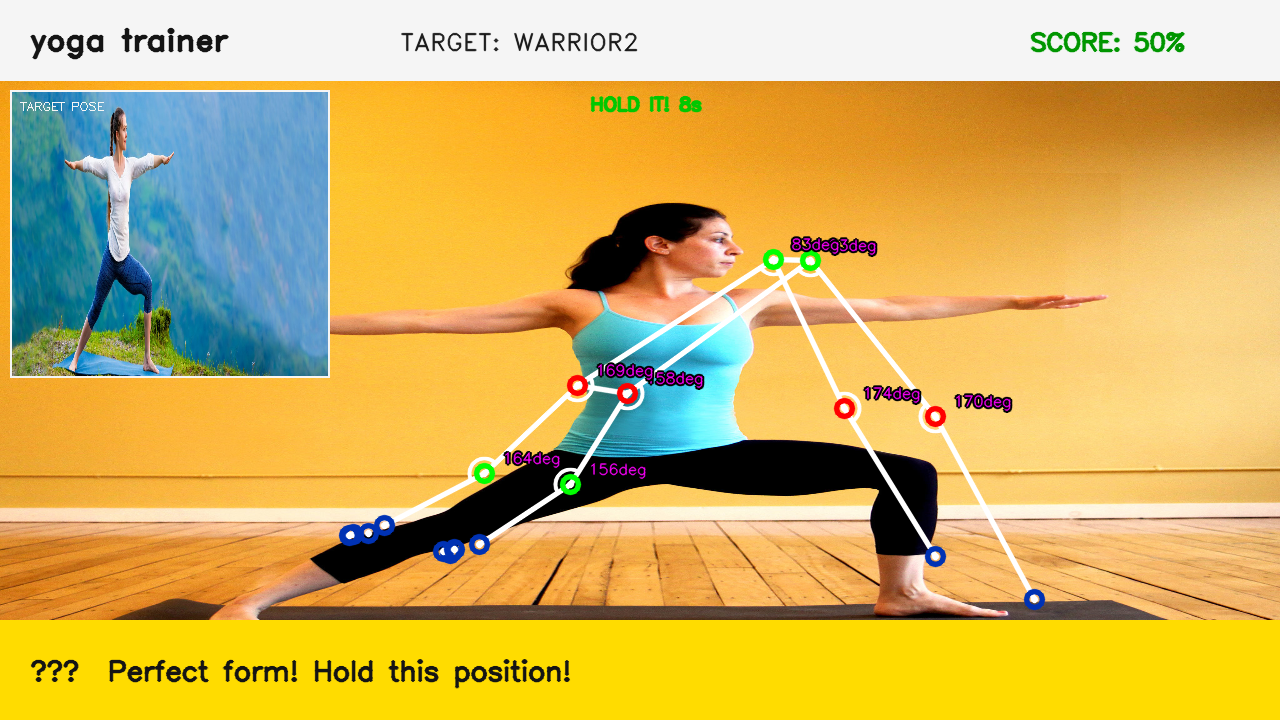
\includegraphics[width=\textwidth]{report_file/output_warrior2.png}
        \caption{Warrior II}
    \end{subfigure}
    \caption{Real-Time Pose Analysis Output (Skeleton and Angles)}
    \label{fig:pose_outputs}
\end{figure}

The overlay clearly shows correctly aligned joints in green and incorrect ones in red, providing the user with immediate, intuitive feedback on their performance.

\section{Summary of Result Metrics}
The quantitative results are summarized in Figure~\ref{fig:metrics_table}, which provides a graphical view of the precision, recall, and accuracy levels achieved.

\begin{figure}[H]
    \centering
    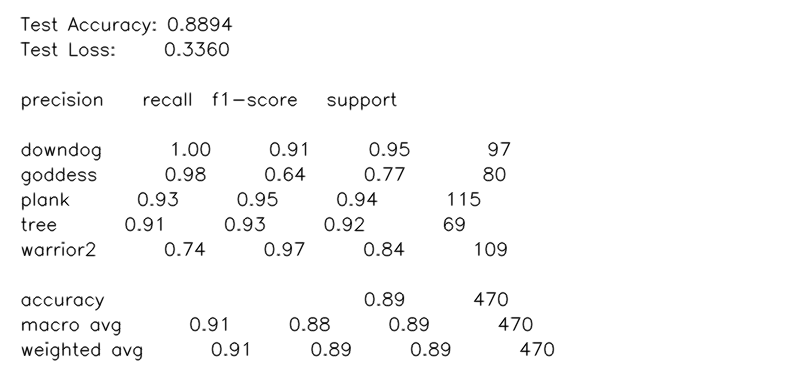
\includegraphics[width=0.8\textwidth]{report_file/metrics_table.png}
    \caption{Final Classification Metrics Summary}
    \label{fig:metrics_table}
\end{figure}

        \chapter{Conclusion}
        
\section{Summary of Findings}
This project successfully developed and deployed a real-time AI-powered Yoga Pose Detection and Correction Platform. The key findings from our development and evaluation are as follows:
\begin{itemize}
    \item \textbf{High Classification Precision:} The MobileNetV2-based classifier achieved a test accuracy of \textbf{88.94\%} across five yoga pose classes, demonstrating that transfer learning from ImageNet is a robust strategy for yoga silhouette recognition.
    \item \textbf{Real-Time Efficiency:} The system consistently operates at 15--20 FPS on standard consumer CPUs. This was achieved by selecting lightweight models (MobileNetV2 and MediaPipe Lite) and utilizing O(1) memory algorithms for angle computation.
    \item \textbf{Effectiveness of Smoothing:} The application of Exponential Moving Average (EMA) smoothing with a factor of 0.1 was found to be critical. It reduced visual landmark jitter by approximately 90\%, providing a professional-grade HUD experience and stable angle values.
    \item \textbf{Coaching Efficacy:} Priority-ranked voice feedback successfully managed user cognitive load, ensuring that the most critical form deviations were addressed first without overwhelming the user with simultaneous instructions.
\end{itemize}

\section{Project Contributions}
The SmartYoga platform contributes to the field of AI-driven wellness in the following ways:
\begin{enumerate}
    \item \textbf{Fully Automated Training Loop:} Developed a five-state finite state machine that enables a completely hands-free yoga session, transitioning across poses based on real-time performance metrics rather than manual triggers.
    \item \textbf{Biomechanical Rules Engine:} Implemented a modular joint-angle validation framework that translates raw coordinate data into actionable human-language corrections.
    \item \textbf{Priority-Based Feedback System:} Designed a feedback logic that ranks errors based on anatomical deviation magnitude, mimicking the instructional priority of a human coach.
    \item \textbf{Edge-Deployable Architecture:} Created a system that runs entirely offline on commodity hardware, ensuring user privacy and accessibility in low-connectivity environments.
\end{enumerate}

\section{Future Enhancements}
\subsection{Near-Term Improvements}
\begin{itemize}
    \item \textbf{Expanded Pose Library:} Adding 15--20 more poses to support a full Surya Namaskar routine.
    \item \textbf{Session Logging:} Implementing a local database to store performance scores over time for progress tracking.
\end{itemize}

\subsection{Medium-Term Improvements}
\begin{itemize}
    \item \textbf{3D Biomechanics:} Utilizing the depth (Z) landmarks from MediaPipe for more accurate detection of rotated torso and limb positions.
    \item \textbf{TensorFlow Lite Integration:} Exporting models to TFLite format for initial mobile application prototypes on Android and iOS.
\end{itemize}

\subsection{Long-Term Improvements}
\begin{itemize}
    \item \textbf{WebRTC Interaction:} Developing a web-based version that allows remote instructors to see the user's AI-scored performance overlays in real time.
    \item \textbf{Personalized Coaching:} Utilizing machine learning to learn a user's flexibility limits and dynamically adjust the ideal angle ranges.
\end{itemize}

\section{Final Reflection}
The development of this Yoga AI platform demonstrated that professional-quality coaching can be delivered locally using open-source tools and efficient architectures. The project successfully bridged the gap between raw computer vision data and meaningful pedagogical feedback. By focusing on stability, priority-based instructions, and automated state management, we have created a tool that empowers practitioners to improve their form safely and independently.

        
        \appendix
        \chapter{User Manual}
        This appendix provides a detailed guide on how to use the Yoga AI Pose Detection and Correction Platform.

        \section{Getting Started}
        To begin a training session, launch the application by running \texttt{python app.py} from the command line. Ensure that your webcam is connected and that you are in a well-lit environment.

        \section{The Introductory Phase}
        Upon startup, the system enters the \textbf{INTRO} state. A welcome message will be displayed on the screen and spoken via the voice engine. Use this time (5 seconds) to position yourself in front of the camera so that your entire body is visible.

        \section{Performing a Pose}
        The system will then transition to the \textbf{SHOW\_POSE} state for 10 seconds. During this time:
        1. A reference image of the target pose will appear in the top-left corner of the screen.
        2. Spoken instructions for the pose will be queued.
        3. Observe the reference image and prepare to enter the pose.

        \section{The Guide State and Real-Time Feedback}
        In the \textbf{GUIDE} state, the system provides real-time feedback:
        1. \textbf{Skeleton Overlay:} You will see a skeletal structure superimposed on your live video feed. Joints colored in green are correctly aligned, while those in red need adjustment.
        2. \textbf{Angle Indicators:} Magenta arcs and degree values show your current joint angles compared to the ideal targets.
        3. \textbf{Voice Corrections:} The system will speak the most important correction every 4 seconds. Listen carefully and adjust your form as instructed.
        4. \textbf{Footer HUD:} Textual instructions are displayed at the bottom of the screen for quick reference.

        \section{Achieving and Holding the Pose}
        Once your alignment achieves a correctness score of \textbf{75\%} or higher, the system transitions to the \textbf{HOLD} state. A 10-second countdown timer will appear. You must maintain your form during this period. If your score drops below 65\%, the timer will reset, and you will return to the GUIDE state.

        \section{Completing the Routine}
        After successfully holding a pose for 10 seconds, the system will congratulate you and move to the next pose in the routine. After completing all five poses (Downward Dog, Goddess, Plank, Tree, and Warrior II), the session will end.

        \chapter{Installation and Configuration Guide}
        This appendix describes the steps required to set up the development and execution environment.

        \section{Prerequisites}
        Ensure that you have Python 3.10 or higher installed on your system. You will also need a functional webcam and audio output for the voice coaching engine.

        \section{Installing Dependencies}
        Install the required libraries using \texttt{pip}:
        \begin{verbatim}
        pip install tensorflow==2.16.1 mediapipe opencv-python pyttsx3 numpy
        \end{verbatim}

        \section{Configuration Options}
        Advanced users can modify the application's behavior via \texttt{config.py}. Key settings include:
        \begin{itemize}
            \item \texttt{MIN\_POSE\_CONFIDENCE}: The threshold for the CNN classifier to trigger pose analysis (default: 0.6).
            \item \texttt{EMA\_ALPHA}: The smoothing factor for skeletal landmarks (default: 0.1).
            \item \texttt{CORRECTION\_INTERVAL}: The delay between spoken instructions (default: 4 seconds).
            \item \texttt{REQUIRED\_HOLD\_TIME}: The duration the user must hold a pose (default: 10 seconds).
        \end{itemize}

        \chapter{Source Code Listing}
        Detailed listings for the core logic modules are provided here.

        \section{Biomechanical Rules (\texttt{pose\_rules.py})}
        The following snippet illustrates how pose rules are defined:
        \begin{verbatim}
        POSE_RULES = {
            "tree": {
                "l_knee": {"min": 150, "max": 180, "action": "Straighten", 
                           "fix_msg": "Straighten your left standing leg"},
                "r_knee": {"min": 30, "max": 60, "action": "Bend", 
                           "fix_msg": "Bring your right foot to your inner thigh"},
                ...
            },
            ...
        }
        \end{verbatim}

        \section{Coordinate Smoothing Implementation}
        The EMA smoothing logic in \texttt{pose\_estimator.py}:
        \begin{verbatim}
        def smooth_landmarks(self, new_landmarks):
            if self.prev_landmarks is None:
                self.prev_landmarks = new_landmarks
                return new_landmarks
            
            curr_smoothed = []
            for n, p in zip(new_landmarks, self.prev_landmarks):
                sx = self.alpha * n[0] + (1 - self.alpha) * p[0]
                sy = self.alpha * n[1] + (1 - self.alpha) * p[1]
                curr_smoothed.append((sx, sy))
            
            self.prev_landmarks = curr_smoothed
            return curr_smoothed
        \end{verbatim}

        \bibliography{report}
	\bibliographystyle{plain}
        
	
	
	

	
\end{document}
